\documentclass[12pt,twoside,openright,a5paper]{book}
\usepackage[margin=0.75in]{geometry}
\usepackage{layout}
\usepackage{pgffor}
\usepackage{tocloft}
\usepackage[table, dvipsnames]{xcolor}
\usepackage{fontspec}
\usepackage{fancybox}
\usepackage[skins]{tcolorbox}
\usepackage{fancyhdr}
\usepackage{setspace}
\usepackage[utf8]{inputenc}
\usepackage{emptypage}
\usepackage[vskip=0pt,rightmargin=0cm]{quoting}
\usepackage{sectsty}
\usepackage{polyglossia}
\usepackage{changepage}%
\usepackage{imakeidx}
\usepackage{setspace}
\usepackage{longtable,array}
\usepackage{tikz} % Package for drawing
\usepackage{tikzpagenodes}
\usepackage[toc,acronym]{glossaries}
\usepackage{fontawesome5}
\usepackage{marvosym}
\usepackage[totoc, font=footnotesize]{idxlayout}
\usepackage{eso-pic} % background image in titlepage
\usepackage{anyfontsize} % any font size
\usepackage{pgfornament} % design package
\usepackage{nextpage}
\usepackage[percent]{overpic}
\usepackage{moresize}




\newfontfamily\engfont[]{Arial}
\usepackage[hpos=24mm,fontsize=32pt, hanchor=l,anchor=lc,angle=90,color={[gray]{0.5}}, text={\engfont{DRAFT \ COPY}}]{draftwatermark}

\newskip\linepagesep \linepagesep 5pt\relax
\renewcommand\footrulewidth{0.5pt}
\def\vfootline{%
    \begingroup
        \color{blue}\rule[-990pt]{20pt}{1000pt}
    \endgroup}



\setmainfont[Script=Devanagari]{Noto Serif Devanagari}
\setmainlanguage{sanskrit}
\setotherlanguages{english}
%\newfontfamily\kannadafont[Script=Kannada]{Noto Serif Devanagari}
%\newfontfamily\kannadafontsf[Script=Kannada]{Noto Serif Devanagari}
%\newfontfamily\devBold[Script=Sanskrit]{Noto Serif Devanagari Bold}
\newfontfamily\devfont[Script=Devanagari]{Sanskrit 2003}
\newfontfamily\mananamfont[]{Arial Rounded MT Bold}
\newfontfamily\mananamtext[]{Monotype Corsiva}
\newfontfamily\meaningtext[]{Arial Narrow}
\newfontfamily\arialUC[]{Arial Unicode MS}
\newfontfamily\selfReflect[]{Arial Rounded MT Bold}
\newfontfamily\devanagarifont[]{Noto Serif Devanagari}
%\newfontfamily\akayaKan[Script=Kannada]{Akaya Kanadaka}
\newfontfamily\devanagarifontsf{Noto Serif Devanagari}
\newfontfamily\devanagarifonttt{Sanskrit 2003}
\fancyhf{}
  \fancyfoot[RO]{\vfootline\hskip\linepagesep\thepage}
  \fancyfoot[LE]{\thepage\hskip\linepagesep\vfootline}
  \fancyhead[RO]{\footnotesize \devfont गीतामननम्} %Odd page Right
  \fancyhead[LO]{\footnotesize \devfont दिनाङ्क ..../..../.....} % Odd page Left
  \fancyhead[LE]{\footnotesize \devfont गीतामननम्} %Even page Left
  \fancyhead[RE]{\footnotesize \devfont दिनाङ्क ..../..../.....} %Even page Right
  \renewcommand\headrulewidth{1pt}
  \fancypagestyle{plain}{%
    \fancyhf{}
    \fancyfoot[RO]{\vfootline\hskip\linepagesep\thepage}
    \fancyfoot[LE]{\thepage\hskip\linepagesep\vfootline}
    \renewcommand\headrulewidth{0pt}
  }
\quotingsetup{font={itshape,footnotesize}}


\addto\captionskannada{\renewcommand{\contentsname}{\color{blue}{विशयसूचि}}} 

% Reduce space between TOC
\setlength\cftparskip{-2pt}
\setlength\cftbeforechapskip{2pt}
\setcounter{secnumdepth}{-1}
\chapterfont{\color{blue}}  % sets colour of chapters
\setlength\parindent{0pt} % no-indent for entire file
\date{} % clear date
\makeindex
\indexsetup{othercode=\small}
%\include{./glossaries-kan}
%\makeglossaries


\newcommand\Linepage[1][0.40in]{% Change to suit
  \vbox to \dimexpr\textheight-\pagetotal-#1\relax {% Let TeX do the work...
    \leaders\hbox to \linewidth{\rule{0pt}{#1}\hrulefill}\vfil
  }%
}

\newtcolorbox{inspiration}[2][]{%
  floatplacement=b,float, 
  enhanced,colback=white,colframe=purple,coltitle=black,
  sharp corners,boxrule=1pt, width=\textwidth,
  fonttitle=\sffamily\scshape\color{teal},
  rightrule=3mm,
  fontupper=\itshape,
  fontlower=\tiny,
  attach boxed title to top left={yshift=-0.5\baselineskip-0.4pt,xshift=2mm},
  boxed title style={tile,size=minimal,left=0.5mm,right=0.5mm,
    colback=white,before upper=\strut},
  title=#2,#1
}
\newtcolorbox{mananam}[2][fontlower=\small]{%
  enhanced,colback=white,colframe=teal,coltitle=black,
  sharp corners,boxrule=1pt, width=\textwidth,
  fonttitle=\sffamily\scshape\color{purple},
  leftrule=3mm,
  fontupper=\itshape,
  fontlower=\tiny,
  attach boxed title to top left={yshift=-0.5\baselineskip-0.4pt,xshift=4mm},
  boxed title style={tile,size=minimal,left=0.5mm,right=0.5mm,
    colback=white,before upper=\strut},
  title=#2,#1
}

\newcommand\Index[1]{#1\index{#1}}


% commands
\definecolor{aurometalsaurus}{rgb}{0.43, 0.5, 0.5}
\newcommand{\slcol}[1]{{\large\color{Blue}{#1}}}
\newcommand{\cquote}[1]{\begin{quoting}[vskip=5pt]{\color{black}{\meaningtext #1}}\end{quoting}}
\newcommand{\translate}[1]{\begin{quoting}[vskip=3pt]{\color{blue}{\arialUC #1}}\end{quoting}}
%\input{./index-page}
\renewcommand{\cftchapfont}{\normalfont}
\renewcommand{\cftchappagefont}{\normalfont}
%column decoration
\setlength{\columnseprule}{1pt}
\def\columnseprulecolor{\color{blue}}

\begin{document}

\pagenumbering{roman}
\begin{titlepage}
	%\pagecolor{pastelblue}
	\AddToShipoutPictureBG*{%
    \AtPageLowerLeft{%
        \includegraphics[width=\paperwidth,height=\paperheight]{../images/krishna4.jpg}%
    }%
}
    \begin{center}
        \vspace*{-1.5cm}
        {\HUGE \textbf{\devfont{\color{white} गीतामननम्}}}\\
        {\normalsize\textbf{\devfont{\color{white}दैनिकजीवनाय प्रेरणाय च}}}\\
        \vspace{1.0cm}    
        \textbf{{\Large \color{white}\devfont स्वामि निर्गुणानन्द गिरि}}
        %\textbf{\\ \small \color{white}ದೈನಂದಿನ ಸ್ಪೂರ್ತಿ ಹಾಗೂ ಆತ್ಮಾವಲೋಕನಕ್ಕಾಗಿ}    
        \vspace{0.0cm}
            
        
		
            
        \vfill
            
        
            
        \vspace{0.1cm}
        {\Large \textbf{\color{white}\devfont संपुट - १}\\}
        \small\color{white}\devfont (अध्याय १ - ६)\\
        {\color{white}    
		%\textbf{{\Large \mananamfont ಸ್ವಾಮಿ ನಿರ್ಗುಣಾನಂದ ಗಿರಿ}}\\
		%{\normalsize Swami Nirgunananda Giri\\Rishikesh, India}
		}
    \end{center}
\end{titlepage}
\nopagecolor% Use this to restore the color pages to white
\begin{titlepage}
	%\pagecolor{pastelblue}
	%\AddToShipoutPictureBG*{%
    %\AtPageLowerLeft{%
    %    \includegraphics[width=\paperwidth,height=\paperheight]{./images/krishna4.jpg}%
    %}%
%}
    \begin{center}
        \vspace*{0.5cm}
            
        {\HUGE
        \textbf{\color{blue}\fontsize{50}{60}\devfont गीतामननम्}}
        \textbf{\\ \devfont \color{black}दैनिकजीवनाय प्रेरणाय च}\\ 
		\vspace{1.0cm}
		\textbf{{\large \devfont\color{black} संपुट - १}\\{\normalsize \devfont\color{black} (अध्याय १ - ६)}}\\		
        \vspace{6.0cm}
        \textbf{{\Large \color{blue}\devfont स्वामि निर्गुणानन्द गिरि}}\\    
        
		
            
        \vfill
            
        
            
        \vspace{0.1cm}
        {\color{black}    
		
		{{\large \devfont\color{blue} ऋषिकेश, उत्तराखण्ड}\\\normalsize भारत}
        }
    \end{center}
\end{titlepage}
\nopagecolor% Use this to restore the color pages to white
%\maketitle

\thispagestyle{empty}
Copyright \textcopyright\ Swami Nirgunananda Giri\\
\\
All rights reserved\\
\\
Edition - First, 2025\\
Sample Copy, Not for Sale\\
\vfill
Without written permission of the author it is forbidden to reproduce or adapt in any form or by any means any part of this  publication.\\
\\
Rishikesh, India\\
\newpage
\thispagestyle{empty}
\frontmatter

\doublespacing
\tableofcontents
\singlespacing
%\clearpage
%\newgeometry{margin=0pt} % Apply margin only for this page
%\thispagestyle{empty}
%\begin{center}
%\includegraphics[width=0.9\textwidth, height=\paperheight, keepaspectratio]{./images/ganapa.jpg}
%\end{center}
%\restoregeometry % Restore original geometry settings
%\newpage

\clearpage
\newgeometry{margin=0pt} % Apply margin only for this page
\thispagestyle{empty}
%\begin{figure}
%\centering
%\includegraphics[width=0.9\textwidth, height=\paperheight, keepaspectratio]{./images/ganapa.jpg}
%\includegraphics[width=\paperwidth, height=\paperheight]{./images/ganapa.jpg}
%\end{figure}
%\restoregeometry % Restore original geometry settings
%\newpage

\begin{figure}[h!]
    \centering
    \begin{overpic}[width=\paperwidth, height=\paperheight]{../images/001.jpg}
        \put(17,85){\color{white}\devfont गजाननं भूतगणादि सेवितं कपित्थजम्बूफलसार भक्षितम् ।
        }
        \put(17,82){\color{white}\devfont उमासुतं शोकविनाशकारणं नमामि विघ्नेश्वर पादपङ्कजम् ॥}
    \end{overpic}
    \caption{This is the standard figure caption below the image.}
    \label{fig:example}
\end{figure}

\restoregeometry

\thispagestyle{empty}
\thispagestyle{empty}
\pagestyle{fancy}


\chapter{Preface}
\begin{center}
\large\devfont दिशन्तु शं मे गुरुपादपांसवः
\end{center}

{\small
Srimad Bhagavad Gita is a unique and unparalleled jewel among all scriptures. It serves as a guiding light not only for renunciants but also for those laden with worldly responsibilities, attempting to balance the material with the spiritual. It advocates them to be impartial in the dealings of their body and mind, which out of ignorance they get identified with. It is a wrong notion that in order to accomplish one's duties in life, a sense of attachment is necessary. Lord Krishna, the biggest संसारी (samsari) of all is a perfect unattached असंसारी (asamsari). He demonstrates through his actions and words as to how to function in this tangible, material world while being grounded in the sublime bliss.\\


To attain this state, one needs proper guidance from capable teachers who show the path that initially appears to be conflicting and full of challenges. As pointed out by the deep insight of the author of this master guide book  in verses 52-53 of Ch 2:
"The purpose of the teacher and scriptures is to shake us out of delusion. Confusions and challenges are a part of spiritual journey as we let go of our worldly thinking patterns and seek refuge in the higher reality. As we thus progress, we begin to gain clarity on the path."\\


This book leads the readers, through the author's revolutionary contemplations, from body to mind and from mind to consciousness, penetrating the layers of one's existence. The introspective questions under the title Mananam in each section give no respite to those who are engaged in self appeasement and self-deceit (आत्म प्रवञ्चना) and challenges them towards a honest self-assessment. On the other hand, the words under Inspiration serves as an inexhaustable source of positivity making the arduous and confusing spiritual path relatively easier.\\


This handbook gives ample material for aspirants to find solution to the various issues of life, not outwardly but within oneself. The content of this book shows the profound understanding of the author on the human psychology, progressing first to a positive mental state and then beyond it, to the innermost eternal Self. As the readers of this book embark on this journey, they are certain to surpass the domain of human mind and arrive at the अधिष्ठान चैतन्यम् (ultimate substratum of sentiency), by the grace of the singer of this celestial song, "भगवद्गीता".\\


May the selfless effort of Swami Nirgunanda Giri ji in penning his thougts for the benefit of the seekers be blessed by the Eternal Teacher, Lord Krishna.\\
}
\begin{center}
\devfont मङ्गलम्  सर्वम्
\end{center}

{\large\devfont स्वामी स्वानन्द तीर्थ\\}
\devfont आचार्य, कैलास आश्रम\\
\devfont ऋषिकेश - उत्तराखण्ड
\newpage

%\thispagestyle{empty}
\begin{onehalfspace}
\chapter{Introduction}
\mananamtext{\indent ನಾವೆಲ್ಲರೂ ಜೀವನದ ಹೋರಾಟಗಳನ್ನು ಎದುರಿಸಲೇಬೇಕು. ಕುರುಕ್ಷೇತ್ರ ಯುದ್ಧದಲ್ಲಿ ಶ್ರೀ ಕೃಷ್ಣ ಪರಮಾತ್ಮನು, ತನ್ನ ವೇದನಾಯುಕ್ತ ಶಿಷ್ಯ ಅರ್ಜುನನಿಗೆ, ಪ್ರಾಪಂಚಿಕತೆಯಲ್ಲಿಯೂ ಅಧ್ಯಾತ್ಮಿಕತೆಯನ್ನು ಆಚರಣೆಗೆ ತರುವಂತಹ , ಸಂಕ್ಷಿಪ್ತ ಹಾಗೂ ಪ್ರಾಯೋಗಿಕವಾದ,  ಅತೀ ಪವಿತ್ರವಾದ ಬೋಧನೆಗಳನ್ನು ಕೊಟ್ಟಿದ್ದಾನೆ. ಈ ಶ್ರೇಷ್ಠವಾದ ಉಪನಿಷತ್ತುಗಳ ಸತ್ವಗಳನ್ನೊಳಗೊಂಡ  ಬೋಧನೆಗಳನ್ನು ಪವಿತ್ರವಾದ, ‘ಭಗವದ್ಗೀತ, ಒಂದು ಪವಿತ್ರ ಗಾನ’ ದ ಸ್ವರೂಪದಲ್ಲಿ, ಋಷಿ ವೇದವ್ಯಾಸರು ನಮಗೆ ನೀಡಿರುವ ಅಸೀಮವಾದ ಕೊಡುಗೆ. \\\\
\emph{ಅರ್ಜುನನು ಇದ್ದ ಪರಿಸ್ಥಿತಿಗೂ, ನಾವು ಇರುವ ಪರಿಸ್ಥಿತಿ ಮತ್ತು ಸಂಘರ್ಷಗಳಿಗೂ ವ್ಯತ್ಯಾಸಗಳಿರಬಹುದು. ಆದರೆ, ಗೀತೆಯ ಸಾರ್ವತ್ರಿಕ ಉಪದೇಶಗಳು ಸತ್ಯಾನ್ವೇಷಣೆ ಮಾಡಲು ಬಯಸುವ ಪ್ರಯೊಬ್ಬನಿಗೂ ಆತ್ಮೋನ್ನತಿ  ಮತ್ತು ಅಧ್ಯಾತ್ಮಿಕ ಪ್ರಗತಿ ಸಾಧಿಸಲು ಬೇಕಾಗುವ ಮಾದರಿಯಾಗಿದೆ.\\\\}
ಭಗವದ್ಗೀತೆಯ ಉಪದೇಶಗಳು ಕೇವಲ ಆಧ್ಯಾತ್ಮಿಕ ಅನ್ವೇಷಣೆ ಮಾಡುವವರಿಗೆ ಸಮರ್ಪಿತವಾದದ್ದು ಮಾತ್ರವೇ ಅಲ್ಲ, ಜೀವನಕ್ಕೆ ಬೇಕಾಗುವ ಅತ್ಯಮೂಲ್ಯವಾದ ಕೈಪಿಡಿಯೂ ಆಗಿದೆ. ಯಾರು, ಕೆಲಸದಲ್ಲಿ ಮತ್ತು ಕೌಟುಂಬಿಕ ಜವಾಬ್ದಾರಿಗಳಲ್ಲಿ ಒತ್ತಡ ರಹಿತವಾಗಿ, ಸಮತೋಲನ ಮತ್ತು ಮಾನಸಿಕ ನೆಮ್ಮದಿ ಕಾಪಾಡಿಕೊಳ್ಳಲು  ಬಯಸುತ್ತಾರೋ ಅವರಿಗೆ ಈ ಬೋಧನೆಗಳು ಬಹಳ ಮಹತ್ವದ್ದಾಗಿರುತ್ತವೆ. \\\\
ಅನೇಕ ಗುರುಗಳು ಮತ್ತು ವಿದ್ವಾಂಸರು ಈಗಾಗಲೇ ಮಾಡಿರುವಂತೆ ಈ ದಿನಚರಿ ಪುಸ್ತಕ ಮತ್ತು ನಿಯತಕಾಲಿಕವು, ಗೀತೆಯ ಬೋಧನೆಗಳನ್ನು ತಿಳಿಸುವ ಪ್ರಯತ್ನ ಅಥವಾ ವ್ಯಾಖ್ಯಾನ ಕೊಡುವುದಾಗಿಲ್ಲ. ಈ ಗೀತಾ ಮನನವು, ಬೋಧನೆಗಳ ಚಿಂತನೆ ಮಾಡುವುದು ಮತ್ತು ಅದನ್ನು ನಮ್ಮ ಸ್ವಂತದ್ದನ್ನಾಗಿ ಅಂದರೆ, ಜೀವನದqqಲ್ಲಿ ಅಳವಡಿಸಿಕೊಳ್ಳಲು ಸುಲಭವಾಗುವಂತೆ ಮಾಡಿಕೊಳ್ಳುವುದೇ ಆಗಿದೆ. ದೇವ ನಾಗರಿಯಲ್ಲಿರುವ `ಮನನ` ಎಂಬ ಪದವು ಆಗಲೇ ಕೇಳಿದ್ದನ್ನು ಅಥವಾ ಓದಿದ್ದನ್ನು ಚಿಂತನೆ ಮಾಡುವ ಕಾರ್ಯವಿಧಾನವನ್ನು ಅನ್ವಯಿಸುವುದಾಗಿದೆ.\\\\
ಈ ದಿನಚರಿ ಪುಸ್ತಕವನ್ನು ನೀವು, ನಿಮ್ಮ ಮನಸ್ಸಿನ ಇಂಗಿತವನ್ನು ಸ್ವತಂತ್ರವಾಗಿ ವ್ಯಕ್ತಪಡಿಸಲು  ಮತ್ತು ನಿಮ್ಮ ಜೀವನದಲ್ಲಿ ಅಳವಡಿಸಿಕೊಳ್ಳಲು ಅವಕಾಶ ಮಾಡಿಕೊಡುವ ಸಲುವಾಗಿ  ರೂಪಿಸಲಾಗಿದೆ. ಗೀತೆಯಲ್ಲಿರುವ ಶ್ಲೋಕಗಳ ಆಧಾರದ ಮೇಲೆ ರಚಿಸಲಾಗಿರುವ ಈ ಪ್ರಶ್ನೆಗಳು, ಆಯಾ ಬೋಧನೆಗಳ ಸನ್ನಿವೇಶಕ್ಕೆ ತಕ್ಕಂತೆ, ನಿಮ್ಮ ವೈಯಕ್ತಿಕ ಅರ್ಥಗಳನ್ನು ಹುಡುಕಲು ಮತ್ತು ಅದರಿಂದ ಜೀವನದ ಸಂದರ್ಭದೊಳಗೆ ಅಪಾರ ಸ್ಪಷ್ಟನೆ ದೊರಕಿಸಲು ಸಹಾಯಕವಾಗುವಂತೆ ರೂಪಿಸಲಾಗಿದೆ.
ಶ್ರೀ ಕೃಷ್ಣ ಪರಮಾತ್ಮನು  ಅರ್ಜುನನಿಗೆ ಧಾರ್ಮಿಕ ಯುದ್ಧವನ್ನು ಮಾಡಲು ಪ್ರೇರೇಪಿಸಿದಂತೆ, ನಿಮ್ಮ ಜೀವನದ ದಿನನಿತ್ಯದ ಕರ್ತವ್ಯಗಳನ್ನು ಈ “ಗೀತಾ ಮನನಮ್ “ ಮೂಲಕ  ಸಮರ್ಪಕವಾಗಿ ನಿರ್ವಹಿಸಲು,  ಆ ಭಗವಂತ ನಿಮ್ಮನ್ನೂ ಪ್ರೇರೇಪಿಸುತ್ತಾನೆ ಎಂದು ನಂಬುತ್ತೇನೆ. ನಿಮ್ಮ ಅಂತರಂಗದ ಶಾಂತಿ, ವೈಯಕ್ತಿಕ ಪ್ರಗತಿಯನ್ನು ನಿರ್ಲಕ್ಷಿಸದೇ, ನಿಮ್ಮ ಕರ್ತವ್ಯಗಳನ್ನು ಕುಶಲತೆಯಿಂದ ಯಶಸ್ವಿಯಾಗಿ ನಿರ್ವಹಿಸುತ್ತಾ  ಮತ್ತು ನಿಶ್ಚಲವಾಗಿ ದೈವತ್ವದಲ್ಲಿ ಮನಸನ್ನಿಡುವುದೇ, ಈ ದಿವ್ಯವಾದ ಗೀತೆಯ ನಿರಂತರ ಉದ್ದೇಶ.\\\\
ನಾನು ಈ ಪುಸ್ತಕದಲ್ಲಿ ಬಳಸಿರುವ ಚಿತ್ರಕಲೆ ಮತ್ತು ರೇಖಾಚಿತ್ರಗಳಿಗಾಗಿ ------ ಅವರಿಗೆ ಧನ್ಯವಾದಗಳನ್ನು ಸಲ್ಲಿಸುತ್ತೇನೆ. ಮುದ್ರಣ ಕಾರ್ಯದಲ್ಲಿ ಸಹಾಯ ಮಾಡಿದ -----ಅವರಿಗೆ ನಾನು ಕೃತಜ್ಞತೆ ವ್ಯಕ್ತಪಡಿಸುತ್ತೇನೆ. ನನ್ನ ಗೀತಾ ತರಗತಿಯಲ್ಲಿ ಭಾಗವಹಿಸಿದ್ದ ಅನೇಕ ವಿದ್ಯಾರ್ಥಿಗಳು ಶ್ಲೋಕಗಳ ಭಾಷಾಂತರ, ತಿದ್ದುವಿಕೆ, ಸಂಪಾದನೆ, ವಿನ್ಯಾಸ ಮತ್ತು ಮುದ್ರಣ ಪ್ರಕ್ರಿಯೆಯನ್ನು ಗಮನಿಸುವಲ್ಲಿ ತೊಡಗಿಸಿಕೊಂಡಿದ್ದಾರೆ. ಈ ಗ್ರಂಥವನ್ನು ಓದುಗರ ಹಿತಾರ್ಥಕ್ಕಾಗಿ ಸಮರ್ಪಣೆಯಿಂದ ಮಾಡಿದ ಅವರ ತ್ಯಾಗಮಯ ಸೇವೆಗೆ ಭಗವಂತನ ಕೃಪೆ ಹಾಗು ನನ್ನ ಆಶೀರ್ವಾದಗಳು. }

\end{onehalfspace}
\mainmatter
\pagenumbering{arabic}
\chapter{\devfont १ अर्जुन विशादयोग}
\slcol{धृतराष्ट्र उवाच ।\\
\Index{धर्मक्षेत्रे कुरुक्षेत्रे} समवेता  युयुत्सवः।\\
मामकाः पाण्डवाश्चैव किमकुर्वत सञ्ज्य  ॥१.१॥}
\translate{
  dhṛtarāṣṭra uvāca\\
  dharmākṣētrē kurukṣētrē samavētā yuyutsavaḥ।\\
  māmakāḥ pāṇḍavāścaiva kimakurvata sañjaya॥1.1॥  
}
\cquote{
Dhrtarastra said:
O Sanjaya, on this holy land of Kurushketra, when my people and the Pandavas have gathered eager to fight the battle, what did they do?\\}
\slcol{सञ्जय उवाच ।\\
\Index{दृष्टवा  तु   पाण्डवानीकं}   व्यूढं  दुर्योधनस्तदा ।\\
आचार्यमुपसङ्गम्य  राजा वचनमब्रवीत्  ॥१.२॥}
\translate{sañjaya uvāca\\
dṛṣṭvā tu pāṇḍavānīkaṃ vyūḍhaṃ duryōdhanastadā।\\
ācāryamupasaṅgamya rājā vacanamabravīt॥1.2॥
}
\cquote{Sanjaya said: After observing the Pandava army arranged in military formation, King Duryodhana approached his teacher, Dronacharya, and spoke these words.\\}
\slcol{\Index{पश्यैतां पाण्डुपुत्राणामाचार्य} महतीं चमूम् ।\\
 व्यूढां द्रुपदपुत्रेण तव शिष्येण धीमता ॥१.३॥}
\translate{paśyaitāṃ pāṇḍuputrāṇāmācārya mahatīṃ camūm।\\
vyūḍhāṃ drupadaputrēṇa tava śiṣyēṇa dhīmatā॥1.3॥
}

\newpage

\begin{mananam}{\mananamfont Mananam sloka - 1}
\mananamtext In my everyday life, when my body identified tendencies such as desires, anger, fear, jealousy, etc, were challenged by my deeper urge for freedom and the wisdom gathered from scriptures and teachers, which force did I choose to follow?
\end{mananam}
\WritingHand\enspace{\selfReflect\small{Self Reflection}}
\begin{inspiration}{\mananamfont Inspiration}
\mananamtext Be true to yourself and you will change for the better. Impartial observation is an essential life-skill.\\
It is not enough to simply wish for self-improvement. One must Introspect daily on their thoughts, words, and actions. 
\end{inspiration}
\newpage

\cquote{Behold, O Teacher, at this mighty army of the sons of Pandu, strategically arranged by your wise disciple, the son of Drupada.}
\slcol{\Index{अत्र शूरा महेष्वासा} भीमार्जुनसमा युधि ।\\
युयुधानो विराटश्च द्रुपदश्च महारथः  ॥१.४॥}
\translate{
  atra  śūrā maheṣvāsā bhīmārjunasamā yudhi।\\    
  yuyudhāno virāṭaśca drupadaśca mahārathaḥ॥1.4॥  
}
\cquote{Here, in this army are great warriors like Yuyudhana, Virata, and Drupada, heroic bowmen who are equal in prowess to Bhima and Arjuna.}
\slcol{\Index{धृष्टकेतुश्चेकितानः} काशिराजश्च वीर्यवान्।\\
पुरुजित् कुन्तिभोजश्च् शैब्यश्च नरपुङ्गवः॥१.५॥}
\translate{
dhṛṣṭaketuścekitānaḥ  kāśirājaśca vīryavān।\\
purujit  kuntibhojaśca śaibyśca narapuṅgavaḥ॥1.5॥
}
\cquote{Here are the mighty warriors - Dhrishtaketu, Chekitana, and the valiant king of Kasi; Purujit, Kuntibhoja, and the noble king Shibya.}
\slcol{\Index{युधामन्युश्च विक्रान्त} उत्तमौजाश्च वीर्यवान ।\\
सौभद्रो द्रौपदेयाश्च सर्व एव महारथाः ॥१.६॥}
\translate{
yudhāmanyuśca vikrānta uttamaujāśca vīryavān।\\
saubhadrō draupadēyāśca sarva ēva mahārathāḥ॥1.6॥
}
\cquote{There are the brave Yudhamanyu, the valiant Uttamaujas, the son of Subhadra, and the sons of Draupadi - all great chariot-warriors.}
\slcol{\Index{अस्माकं तु विशिष्टा} ये तान्निबोध द्विजोत्तं ।\\
नायका मम सैन्यस्य संज्ञार्थं ब्रवीमि ते ॥१.७॥}
\translate{
asmākaṃ tu viśiṣṭā yē tānnibōdha dvijōttama।\\
nāyakā mama sainyasya saṃjñārthaṃ tān bravīmi tē॥1.7॥
}
\cquote{O best among the twice-born (Dronacharya),  understand who the distinguished leaders are on our side. I name them to you for your information.}
\slcol{\Index{भवान्भीष्मश्च कर्णश्च} कृपश्च समितिञ्जयः।\\
 अश्वत्थामा विकर्णश्च सौमदत्तिर्जयद्रथः॥१.८॥}
 \translate{
bhavānbhīṣmaśca karṇaśca kr̥paśca samitiñjayaḥ।\\
aśvatthāmā vikarṇaśca saumadattirjayadrathaḥ॥1.8॥ 
 }
\cquote{The victorious in war are Yourself, Bhishma, Karna, and Kripa. Also Ashvatthama, vikarna and Bhurisravas (the son of Somadatta).}
\slcol{\Index{अन्ये च बहवः} शूरा मदर्थे त्यक्तजीविताः ।\\
 नानाशस्त्रप्रहरणाः सर्वे युद्धविशारदाः ॥१.९॥}
\translate{
anyē ca bahavaḥ śūrā madarthē tyaktajīvitāḥ।\\
nānāśastrapraharaṇāḥ sarvē yuddhaviśāradāḥ ॥1.9॥ 
}
\cquote{Furthermore, there are many heroic warriors who are prepared to give up their lives for my sake. They are equipped with various weapons and are all skilled in the art of warfare.}
\slcol{\Index{अपर्याप्तं तदस्माकं} बलं भीष्माभिरक्षितम् ।\\
 पर्याप्तं त्विदमेतेषां बलं भीमाभिरक्षितम् ॥१.१०॥}
\translate{
aparyāptaṁ tadasmākaṁ balaṁ bhīṣmābhirakṣitam।\\
paryāptaṁ tvidamētēṣāṁ balaṁ bhīmābhirakṣitam॥1.10॥ 
 }
\cquote{Our army, protected by Bhishma, is immeasurable. However, this army (the Pandavas’ army), protected by Bhima, is limited.}
\slcol{\Index{अयनेषु च सर्वेषु} यथाभागमवस्थिताः।\\
 भीष्ममेवाभिरक्षन्तु भवन्तः सर्व एव हि॥१.११॥} 
\translate{
ayanēṣu ca sarvēṣu yathābhāgamavasthitāḥ।\\
bhīṣmamēvābhirakṣantu bhavantaḥ sarva ēva hi॥1.11॥ 
}
\cquote{Therefore, all of you, stationed at your respective positions, must support and protect Bhishma from all sides.}
\slcol{\Index{तस्य सञ्जनयन्हर्षं} कुरुवृद्धः पितामहः।\\
 सिंहनादं विनद्योच्चैः शङ्खं दध्मौ प्रतापवान्॥१.१२॥}
\translate{
tasya sañjanayanharṣaṁ kuruvr̥ddhaḥ pitāmahaḥ।\\
siṁhanādaṁ vinadyōccaiḥ śaṅkhaṁ dadhmau pratāpavān॥1.12॥}
\cquote{Then, causing joy in Duryodhana, the mighty grandfather and eldest of the Kuru dynasty, Bhisma, roared like a lion and blew his conch shell loudly.}
\slcol{\Index{ततः शङ्खाश्च} भेर्यश्च पणवानकगोमुखाः।\\
 सहसैवाभ्यहन्यन्त स शब्दस्तुमुलोऽभवत्॥१.१३॥}
\translate{
tataḥ śaṅkhāśca bhēryaśca paṇavānakagōmukhāḥ।\\
sahasaivābhyahanyanta sa śabdastumulō:'bhavat॥1.13॥ 
}
\cquote{Thereafter, conch shells, kettledrums, tabors (small drum), and cow-horns (a musical instrument), immediately resounded together, creating an enormous noise.}
\slcol{\Index{ततः श्वेतैर्हयैर्युक्ते} महति स्यन्दने स्थितौ।\\
 माधवः पाण्डवश्चैव दिव्यौ शङ्खौ प्रदध्मतुः॥१.१४॥}
\translate{
tataḥ śvētairhayairyuktē mahati syandanē sthitau।\\
mādhavaḥ pāṇḍavaścaiva divyau śaṅkhau pradadhmatuḥ॥1.14॥ 
}
\cquote{Then, Krishna (Madhava) and Arjuna (Pandava), positioned on their grand chariot pulled by white horses, blew their divine conch shells.}
\slcol{\Index{पाञ्चजन्यं हृषीकेशो} देवदत्तं धनञ्जयः ।\\
पौण्ड्रं दध्मौ महाशङ्खं भीमकर्मा वृकोदरः ॥१.१५॥}
\translate{
pāñcajanyaṁ hr̥ṣīkēśō dēvadattaṁ dhanañjayaḥ।\\
pauṇḍraṁ dadhmau mahāśaṅkhaṁ bhīmakarmā vr̥kōdaraḥ॥1.15॥}
\cquote{Hrisikesha (Krishna) blew the conch named Pancajanya, while Dhanajnaya (Arjuna) blew his conch named Devadatta. Vrikodara (Bhima), known for his great deeds, blew his mighty conch named Paundra.}
\slcol{\Index{अनन्तविजयं राजा} कुन्तीपुत्रो युधिष्ठिरः।\\
नकुलः सहदेवश्च सुघोषमणिपुष्पकौ॥१.१६॥}
\cquote{King Yudhishthira, the son of Kunti, blew the conch named Anatavijaya, while Nakula and Sahadeva blew their conches named Sughosha and Manipuspaka, respectively.}
\slcol{\Index{काश्यश्च परमेष्वासः} शिखण्डी च महारथः ।\\
धृष्टद्युम्नो विराटश्च सात्यकिश्चापराजितः ॥१.१७॥}
\translate{
kāśyaśca paramēṣvāsaḥ śikhaṇḍī ca mahārathaḥ।\\
dhr̥ṣṭadyumnō virāṭaśca sātyakiścāparājitaḥ॥1.17॥
}
\cquote{Kashya, the supreme archer; Sikhandi, the great warrior; Dhrishtadyumna, Virata and Satyaki (Yuyudhana), who is undefeated.} 
\slcol{\Index{द्रुपदो द्रौपदेयाश्च} सर्वशः पृथिवीपते।\\
सौभद्रश्च महाबाहुः शङ्खान्दध्मुः पृथक्पृथक्॥१.१८॥}
\translate{
drupadō draupadēyāśca sarvaśaḥ pr̥thivīpatē।\\
saubhadraśca mahābāhuḥ śaṅkhāndadhmuḥ pr̥thakpr̥thak॥1.18॥}
\cquote{O King of the Earth, Drupada, and the sons of Draupadi, and the son of Subhadra, one with great arms, blew their conches.}
\slcol{\Index{स घोषो धार्तराष्ट्राणां} हृदयानि व्यदारयत् ।\\
नभश्च पृथिवीं चैव तुमुलो व्यनुनादयन् ॥१.१९॥}
\translate{
sa ghōṣō dhārtarāṣṭrāṇāṁ hr̥dayāni vyadārayat।\\
nabhaśca pr̥thivīṁ caiva tumulō vyanunādayan॥1.19॥
}
\cquote{The sound of these conch shells vibrated in the hearts of Dhritarashtra’s sons, and their uproarious noise echoed through the sky and the earth.}
\slcol{\Index{अथ व्यवस्थितान्दृष्ट्वा} धार्तराष्ट्रान्कपिध्वजः ।\\
प्रवृत्ते शस्त्रसम्पाते धनुरुद्यम्य पाण्डवः ॥१.२०॥\\
\Index{हृषीकेशं तदा} वाक्यमिदमाह महीपते ।}
\translate{
pravr̥ttē śastrasampātē dhanurudyamya pāṇḍavaḥ॥1.20॥\\
hr̥ṣīkēśaṁ tadā vākyamidamāha mahīpatē।
}
\cquote{Then, O King, after observing Dhritarashtra’s sons positioned in military formation, Arjuna, whose flag bore the emblem of Hanuman, lifted his bow as the conflict was about to begin and spoke the following words to Hrishikesha (Krishna).}
\slcol{अर्जुन उवाच —\\
 सेनयोरुभयोर्मध्ये रथं स्थापय मेऽच्युत ॥ १.२१ ॥\\
\Index{यावदेतान्निरीक्षेऽहं} योद्धुकामानवस्थितान् ।\\
 कैर्मया सह योद्धव्यमस्मिन्रणसमुद्यमे ॥ १.२२ ॥}
\translate{
arjuna uvāca — \\
sēnayōrubhayōrmadhyē rathaṁ sthāpaya mē:'cyuta॥1.21॥\\
yāvadētānnirīkṣē:'haṁ yōddhukāmānavasthitān।\\
kairmayā saha yōddhavyamasminraṇasamudyamē॥1.22॥
}
\cquote{Arjuna said: O Achyuta (Krishna), please place my chariot in between the two armies, so that I may observe the warriors positioned here for the battle, with whom I must engage with.}
\slcol{\Index{योत्स्यमानानवेक्षेऽहं} य एतेऽत्र समागताः ।\\
धार्तराष्ट्रस्य दुर्बुद्धेर्युद्धे प्रियचिकीर्षवः ॥१.२३॥}
\translate{
yōtsyamānānavēkṣē:'haṁ ya ētē:'tra samāgatāḥ।\\
dhārtarāṣṭrasya durbuddhēryuddhē priyacikīrṣavaḥ॥1.23॥
}
\cquote{For, I wish to see those who have come here to fight and have assembled to support the evil-minded Duryodhana, the son of Dhritarashtra, in this battle.}
\slcol{सञ्जय उवाच —\\
\Index{एवमुक्तो हृषीकेशो} गुडाकेशेन भारत ।\\
सेनयोरुभयोर्मध्ये स्थापयित्वा रथोत्तमम् ॥१.२४॥}
\translate{
sañjaya uvāca —
ēvamuktō hr̥ṣīkēśō guḍākēśēna bhārata।\\
sēnayōrubhayōrmadhyē sthāpayitvā rathōttamam॥1.24॥
}
\cquote{Sanjaya said: O Bharata (Dhritarashtra), after being addressed by Gudakesha (Arjuna), Hrishikesha (Krishna) placed the excellent chariot between the two armies.}
\slcol{\Index{भीष्मद्रोणप्रमुखतः} सर्वेषां च महीक्षिताम् ।\\
उवाच पार्थ पश्यैतान्समवेतान्कुरूनिति ॥१.२५॥}
\translate{
bhīṣmadrōṇapramukhataḥ sarvēṣāṁ ca mahīkṣitām।\\
uvāca pārtha paśyaitānsamavētānkurūniti॥1.25॥
}
\cquote{In front of Bhishma, Drona and all the other warriors of the world, Krishna said “O Partha (Arjuna), look at these Kurus who have assembled here”.}
\slcol{\Index{तत्रापश्यत्स्थितान्पार्थः} पितॄनथ पितामहान् ।\\
आचार्यान्मातुलान्भ्रातॄन्पुत्रान्पौत्रान्सखींस्तथा ॥१.२६॥}
\translate{
tatrāpaśyatsthitānpārthaḥ pitr̥̄natha pitāmahān।\\
ācāryānmātulānbhrātr̥̄nputrānpautrānsakhīṁstathā॥1.26॥
}
\cquote{Then, Partha (Arjuna) saw on the battlefield, his own relatives, including his fathers, grandfathers, teachers, maternal uncles, brothers, sons, grandsons, and friends, all standing there.}
\slcol{\Index{श्वशुरान्सुहृदश्चैव}सेनयोरुभयोरपि ।\\
 तान्समीक्ष्य स कौन्तेयः सर्वान्बन्धूनवस्थितान् ॥१.२७॥\\
\Index{कृपया परयाविष्टो} विषीदन्निदमब्रवीत् ।}
\translate{
śvaśurānsuhr̥daścaivasēnayōrubhayōrapi।\\
tānsamīkṣya sa kauntēyaḥ sarvānbandhūnavasthitān॥1.27॥\\
kr̥payā parayāviṣṭō viṣīdannidamabravīt।
}
\cquote{Seeing his fathers-in-law, friends, and relatives positioned on both sides of the battlefield, Arjuna, overwhelmed with deep compassion and sorrow, spoke the following words.}
\slcol{अर्जुन उवाच —\\ 
दृष्ट्वेमान्स्वजनान्कृष्ण युयुत्सून्समुपस्थितान् ॥१.२८॥}
\translate{
arjuna uvāca —\\
dr̥ṣṭvēmānsvajanānkr̥ṣṇa yuyutsūnsamupasthitān॥1.28॥
}
\cquote{Arjuna said: O Krishna, after seeing these relatives and friends who desire to fight, my mind is overwhelmed with sorrow and compassion.}
\slcol{\Index{सीदन्ति मम गात्राणि} मुखं च परिशुष्यति ।\\
वेपथुश्च शरीरे मे रोमहर्षश्च जायते ॥१.२९॥}
\translate{
sīdanti mama gātrāṇi mukhaṁ ca pariśuṣyati।\\
vēpathuśca śarīrē mē rōmaharṣaśca jāyatē॥1.29॥
}
\cquote{My limbs are failing, my face is drying up, my body trembles, and my hair stands on end.}
\slcol{\Index{गाण्डीवं स्रंसते} हस्तात्त्वक्चैव परिदह्यते ।\\
न च शक्नोम्यवस्थातुं भ्रमतीव च मे मनः ॥१.३०॥}
\translate{
gāṇḍīvaṁ sraṁsatē hastāttvakcaiva paridahyatē।\\
na ca śaknōmyavasthātuṁ bhramatīva ca mē manaḥ॥1.30॥
}
\cquote{O Krishna, seeing my people, gathered here for battle, my limbs fail, and my mouth is parched. My body shivers, and my hair stands on end. My Gandiva-bow slips from my grip, and my skin burns as my mind spins in confusion.}

\newpage
\begin{mananam}{\mananamfont Mananam sloka - 30}
\mananamtext Let me reflect on those moments in life when I had to face tremendous anxiety and was overwhelmed by my outward circumstances. In such situations, was I aware that my physical condition was paralysed due to my mental fears?  
\end{mananam}
\WritingHand\enspace{\selfReflect\small{Self Reflection}}
\begin{inspiration}{\mananamfont Inspiration}
\mananamtext Remain vigilant of your thoughts.Your mental states impact your body.
\end{inspiration}
\newpage

\slcol{\Index{निमित्तानि च पश्यामि} विपरीतानि केशव ।\\
 न च श्रेयोऽनुपश्यामि हत्वा स्वजनमाहवे ॥१.३१॥}
\translate{
nimittāni ca paśyāmi viparītāni kēśava।\\
na ca śrēyō:'nupaśyāmi hatvā svajanamāhavē॥1.31॥
}
\cquote{O Keshava (Krishna), I see only inauspicious omens and adverse signs. I do not perceive any benefit in killing my own kin in this battle.}
\slcol{\Index{न काङ्क्षे विजयं} कृष्ण न च राज्यं सुखानि च ।\\
किं नो राज्येन गोविन्द किं भोगैर्जीवितेन वा ॥१.३२॥}
\translate{
na kāṅkṣē vijayaṁ kr̥ṣṇa na ca rājyaṁ sukhāni ca।\\
kiṁ nō rājyēna gōvinda kiṁ bhōgairjīvitēna vā॥1.32॥
}
\cquote{O Krishna, I desire neither victory, nor kingdom, nor happiness or pleasures. O Govinda, of what use is the kingdom to us? What use are pleasures or even life itself?}
\slcol{\Index{येषामर्थे काङ्क्षितं} नो राज्यं भोगाः सुखानि च।\\
त इमेऽवस्थिता युद्धे प्राणांस्त्यक्त्वा धनानि च॥१.३३॥}
\translate{
yēṣāmarthē kāṅkṣitaṁ nō rājyaṁ bhōgāḥ sukhāni ca।\\
ta imē:'vasthitā yuddhē prāṇāṁstyaktvā dhanāni ca॥1.33॥
}
\cquote{For whose sake we desire the kingdom, pleasures, and happiness, they are all standing here, prepared for battle, having renounced their lives and wealth.}
\slcol{\Index{आचार्याः पितरः} पुत्रास्तथैव च पितामहाः।\\
मातुलाः श्वशुराः पौत्राः स्यालाः सम्बन्धिनस्तथा॥१.३४॥}
\translate{
ācāryāḥ pitaraḥ putrāstathaiva ca pitāmahāḥ।\\
mātulāḥ śvaśurāḥ pautrāḥ syālāḥ sambandhinastathā॥1.34॥
}
\cquote{Teachers, fathers, sons, grandfathers, maternal uncles, fathers-in-law, grandsons, brothers-in-law, and other relatives.}
\slcol{\Index{एतान्न हन्तुमिच्छामि} घ्नतोऽपि मधुसूदन।\\
अपि त्रैलोक्यराज्यस्य हेतोः किं नु महीकृते॥१.३५॥}
\translate{
ētānna hantumicchāmi ghnatō:'pi madhusūdana।\\ 
api trailōkyarājyasya hētōḥ kiṁ nu mahīkr̥tē॥1.35॥
}
\cquote{I do not desire to kill them, even if they attack me, O Madhusudana (Krishna). I have no desire to fight for the sake of the kingdom, even if all the happiness of the three worlds were offered to me. What joy would there be in killing the sons of Dhritarashtra?}
\slcol{\Index{निहत्य धार्तराष्ट्रान्नः} का प्रीतिः स्याज्जनार्दन ।\\
पापमेवाश्रयेदस्मान्हत्वैतानाततायिनः ॥१.३६॥}
\translate{
nihatya dhārtarāṣṭrānnaḥ kā prītiḥ syājjanārdana।\\
pāpamēvāśrayēdasmānhatvaitānātatāyinaḥ॥1.36॥  
}
\cquote{O Janardana (Krishna), what pleasure will we derive from killing the sons of Dhritarashtra? By killing these wrongdoers, sin alone will befall to us.}
\slcol{\Index{तस्मान्नार्हा वयं हन्तुं} धार्तराष्ट्रान्सबान्धवान्।\\
स्वजनं हि कथं हत्वा सुखिनः स्याम माधव ॥१.३७॥}
\translate{
tasmānnārhā vayaṁ hantuṁ dhārtarāṣṭrānsabāndhavān।\\
svajanaṁ hi kathaṁ hatvā sukhinaḥ syāma mādhava॥1.37॥
}
\cquote{Therefore, we cannot destroy our own relatives, the sons of Dhritarashtra, our relatives. How can we be happy, O Madhava, by killing our own kin?}
\slcol{\Index{यद्यप्येते न पश्यन्ति} लोभोपहतचेतसः ।\\
कुलक्षयकृतं दोषं मित्रद्रोहे च पातकम् ॥१.३८॥}
\translate{
yadyapyētē na paśyanti lōbhōpahatacētasaḥ।\\
kulakṣayakr̥taṁ dōṣaṁ mitradrōhē ca pātakam॥1.38॥
}
\cquote{Even if these people, whose minds are veiled by greed, fail to recognize the wrongdoing in the destruction of the family and the sin of betraying friends.}
\slcol{\Index{कथं न ज्ञेयमस्माभिः} पापादस्मान्निवर्तितुम्।\\
कुलक्षयकृतं दोषं प्रपश्यद्भिर्जनार्दन॥१.३९॥}
\translate{
kathaṁ na jñēyamasmābhiḥ pāpādasmānnivartitum।\\
kulakṣayakr̥taṁ dōṣaṁ prapaśyadbhirjanārdana॥1.39॥
}
\cquote{O Janardana (Krishna), how can we fail to recognize that we must avoid this sin? We are witnessing the fault of destroying the family.}
\slcol{\Index{कुलक्षये प्रणश्यन्ति} कुलधर्माः सनातनाः ।\\
धर्मे नष्टे कुलं कृत्स्नमधर्मोऽभिभवत्युत ॥१.४०॥}
\translate{
kulakṣayē praṇaśyanti kuladharmāḥ sanātanāḥ।\\
dharmē naṣṭē kulaṁ kr̥tsnamadharmō:'bhibhavatyuta॥1.40॥
}


\newpage
\begin{mananam}{\mananamfont Mananam sloka - 37}
\mananamtext Have there been times when I justified my actions or inactions due to lack of responsibility? Am I afraid to disassociate myself from those who pull me downward spiritually and negatively influence me, out of a false sense of sympathy?
\end{mananam}
\WritingHand\enspace{\selfReflect\small{Self Reflection}}
\begin{inspiration}{\mananamfont Inspiration}
\mananamtext Rise up to the challenge of life. Take responsibility for your own actions and choices. Mercilessly, get rid of all your negative habits and influences.
\end{inspiration}
\newpage


\cquote{When a family declines, its traditional practices are lost. When righteousness is lost, the entire family is overwhelmed by unrighteousness.}
\slcol{\Index{अधर्माभिभवात्कृष्ण} प्रदुष्यन्ति कुलस्त्रियः ।\\
स्त्रीषु दुष्टासु वार्ष्णेय जायते वर्णसङ्करः ॥१.४१॥}
\translate{
adharmābhibhavātkr̥ṣṇa praduṣyanti kulastriyaḥ।\\
strīṣu duṣṭāsu vārṣṇēya jāyatē varṇasaṅkaraḥ॥1.41॥
}
\cquote{O Krishna, when unrighteousness prevails, the women of the family become corrupted. O Varshneya (descendant of the Vrishni clan), this causes chaos in the caste system (varnasankara) and disrupts the social order.}
\slcol{\Index{सङ्करो नरकायैव} कुलघ्नानां कुलस्य च ।\\
पतन्ति पितरो ह्येषां लुप्तपिण्डोदकक्रियाः ॥१.४२॥}
\translate{
saṅkarō narakāyaiva kulaghnānāṁ kulasya ca।\\
patanti pitarō hyēṣāṁ luptapiṇḍōdakakriyāḥ॥1.42॥
}
\cquote{Such a mix-up leads to hell for those who ruin the family traditions. The ancestors of those who have neglected the rites of offering food and water suffer and fall from grace.}
\slcol{\Index{दोषैरेतैः कुलघ्नानां} वर्णसङ्करकारकैः ।\\
उत्साद्यन्ते जातिधर्माः कुलधर्माश्च शाश्वताः ॥१.४३॥}
\translate{
dōṣairētaiḥ kulaghnānāṁ varṇasaṅkarakārakaiḥ।\\
utsādyantē jātidharmāḥ kuladharmāśca śāśvatāḥ॥1.43॥
}
\cquote{These evil actions, caused by those who destroy families and create disorder in the castes, result in the destruction of traditional duties and timeless family values.}
\slcol{\Index{उत्सन्नकुलधर्माणां} मनुष्याणां जनार्दन ।\\
 नरके नियतं वासो भवतीत्यनुशुश्रुम ॥१.४४॥}
\translate{
utsannakuladharmāṇāṁ manuṣyāṇāṁ janārdana।\\
narakē niyataṁ vāsō bhavatītyanuśuśruma॥1.44॥
}
\cquote{O Janardana (Krishna), we have heard that those who destroy families are destined to dwell in hell permanently. This fate is inevitable for those who bring down their family values.} 
\slcol{\Index{अहो बत महत्पापं} कर्तुं व्यवसिता वयम् ।\\
 यद्राज्यसुखलोभेन हन्तुं स्वजनमुद्यताः ॥१.४५॥}
\translate{
ahō bata mahatpāpaṁ kartuṁ vyavasitā vayam।\\
yadrājyasukhalōbhēna hantuṁ svajanamudyatāḥ॥1.45॥
}
\cquote{Alas! We are about to commit a great sin. We are determined to kill our own kinsmen in order to enjoy the pleasures ruling the kingdom.}
\slcol{\Index{यदि मामप्रतीकारमशस्त्रं} शस्त्रपाणयः ।\\
धार्तराष्ट्रा रणे हन्युस्तन्मे क्षेमतरं भवेत् ॥१.४६॥}
\translate{
yadi māmapratīkāramaśastraṁ śastrapāṇayaḥ।\\
dhārtarāṣṭrā raṇē hanyustanmē kṣēmataraṁ bhavēt॥1.46॥
}
\cquote{If the armed sons of Dhritarashtra were to kill me unarmed and defenseless in the battle, it would be more favorable for me.}
\slcol{सञ्जय उवाच —\\
\Index{एवमुक्त्वार्जुनः सं‍ख्ये} रथोपस्थ उपाविशत् ।\\
विसृज्य सशरं चापं शोकसंविग्नमानसः ॥१.४७॥}
\translate{
ēvamuktvārjunaḥ saṁkhyē rathōpastha upāviśat।\\ 
visr̥jya saśaraṁ cāpaṁ śōkasaṁvignamānasaḥ॥1.47॥
}
\cquote{Sanjaya said: Thus, speaking these words, Arjuna, overwhelmed with sorrow and dejection on the battlefield, took a seat in his chariot and set aside his bow and arrow.}

\begin{center}
इति श्रीमद्भगवद्गीतासूपनिषत्सु  ब्रह्मविद्यायां योगशास्त्रे\\ श्रीकृष्णर्जुनसंवादे अर्जुनविषादयोगो  नाम प्रथमोऽध्यायः ॥
\end{center}




\chapter{\devfont २ साङ्ख्ययोग}
\slcol{सञ्जय उवाच —\\
तं तथा कृपयाविष्टमश्रुपूर्णाकुलेक्षणम्।\\
 विषीदन्तमिदं वाक्यमुवाच मधुसूदनः॥२.१॥}
\translate{sañjaya uvāca —\\
taṁ tathā kr̥payāviṣṭamaśrupūrṇākulēkṣaṇam।\\
viṣīdantamidaṁ vākyamuvāca madhusūdanaḥ॥2.1॥}
\cquote{Sanjaya said: Madhusudana*, seeing Arjuna immersed in sorrow and with eyes soaked in tears of despair, spoke the following words to him with compassion.}
\slcol{श्रीभगवानुवाच —\\
कुतस्त्वा कश्मलमिदं विषमे समुपस्थितम्।\\
 अनार्यजुष्टमस्वर्ग्यमकीर्तिकरमर्जुन॥२.२॥\\}
\translate{śrībhagavānuvāca —\\
kutastvā kaśmalamidaṁ viṣamē samupasthitam।\\
anāryajuṣṭamasvargyamakīrtikaramarjuna॥2.2॥}
\cquote{Sri Bhagavan said: O Arjun, from where has this delusion arisen at this critical juncture? Such unworthy thoughts do not befit an ārya (a noble person); they neither lead to Swarga* nor bring honor but instead bring disgrace.}

\newpage
\slcol{क्लैब्यं मा स्म गमः पार्थ नैतत्त्वय्युपपद्यते।\\
 क्षुद्रं हृदयदौर्बल्यं त्यक्त्वोत्तिष्ठ परन्तप॥२.३॥}
\translate{klaibyaṁ mā sma gamaḥ pārtha naitattvayyupapadyatē।\\
kṣudraṁ hr̥dayadaurbalyaṁ tyaktvōttiṣṭha parantapa॥2.3॥}
\cquote{O Partha* (Arjuna), do not succumb to this weakness, which is unworthy of you. Cast aside this timid apprehension and rise, O Parantapa*!}
\slcol{अर्जुन उवाच —\\
कथं भीष्ममहं सं‍ख्ये द्रोणं च मधुसूदन।\\
इषुभिः प्रतियोत्स्यामि पूजार्हावरिसूदन॥२.४॥}
\translate{arjuna uvāca —\\
kathaṁ bhīṣmamahaṁ saṁ‍khyē drōṇaṁ ca madhusūdana।\\
iṣubhiḥ pratiyōtsyāmi pūjārhāvarisūdana॥2.4॥}
\cquote{Arjuna said: O Madhusudana, how can I face Bhisma and Drona in battle, who are worthy of my worship? O Arisudana* (Krishna), how can I confront them with arrows?}
\slcol{गुरूनहत्वा हि महानुभावान् श्रेयो भोक्तुं भैक्षमपीह लोके।\\
 हत्वार्थकामांस्तु गुरूनिहैव भुञ्जीय भोगान्रुधिरप्रदिग्धान्॥२.५॥}
\translate{gurūnahatvā hi mahānubhāvān śrēyō \\
\hspace*{0.5cm}bhōktuṁ bhaikṣamapīha lōkē।\\
hatvārthakāmāṁstu gurūnihaiva \\
\hspace*{0.5cm}bhuñjīya bhōgānrudhirapradigdhān॥2.5॥}
\cquote{It is indeed better in this world to sustain oneself through alms than to slay these noble teachers. However, by killing them, I would be enjoying worldly pleasures stained with their blood.}
\slcol{न चैतद्विद्मः कतरन्नो गरीयो यद्वा जयेम यदि वा नो जयेयुः।\\
यानेव हत्वा न जिजीविषामस्तेऽवस्थिताः प्रमुखे धार्तराष्ट्राः॥२.६॥}
\translate{na caitadvidmaḥ katarannō garīyō\\
\hspace*{0.5cm}yadvā jayēma yadi vā nō jayēyuḥ।\\
yānēva hatvā na jijīviṣāmastē\\
\hspace*{0.5cm}vasthitāḥ pramukhē dhārtarāṣṭrāḥ॥2.6॥}


\newpage
\begin{mananam}{\mananamfont Mananam sloka - 3}
\mananamtext Do I tend to wallow in self-pity? Do certain outer conditions or inner urges pull down my energies, causing me to yield to my weaknesses? Am I overly sensitive to constructive criticism from teachers or well-meaning friends?
Do I easily give up on my goals and resolutions? What do I need to do to make the intended changes in my life? 
\end{mananam}
\WritingHand\enspace{\selfReflect\small{Self Reflection}}
\begin{inspiration}{\mananamfont Inspiration}
\mananamtext You are never too weak to face your challenges. Don’t give in to doubts, self-pity and temptations. Arise and pursue your highest goals and aspirations. With firm determination, you will find the positive forces of the universe supporting and strengthening you.
\end{inspiration}
\newpage

\cquote{It is unclear which is more favorable - our victory or theirs. The sons of Dhritarashtra stand before us, and living after slaying them would hold no meaning for us.}
\slcol{कार्पण्यदोषोपहतस्वभावः \\
\hspace*{1.0cm} पृच्छामि त्वां धर्मसंमूढचेताः।\\
यच्छ्रेयः स्यान्निश्चितं ब्रूहि तन्मे शिष्यस्तेऽहं \\
\hspace*{1.0cm} शाधि मां त्वां प्रपन्नम्॥२.७॥}
\translate{kārpaṇyadōṣōpahatasvabhāvaḥ\\
\hspace*{0.5cm} pr̥cchāmi tvāṁ dharmasaṁmūḍhacētāḥ।\\
yacchrēyaḥ syānniścitaṁ brūhi tanmē\\
\hspace*{0.5cm} śiṣyastēhaṁ śādhi māṁ tvāṁ prapannam॥2.7॥}
\cquote{My heart is clouded by the weakness, and I am perplexed about what is Dharma*. I request you to clarify what would be Shreyas* for me. I am your disciple, surrendered to you; please wisdom me.}
\slcol{न हि प्रपश्यामि ममापनुद्याद्यच्छोकमुच्छोषणमिन्द्रियाणाम्।\\
 अवाप्य भूमावसपत्नमृद्धं राज्यं सुराणामपि चाधिपत्यम्॥२.८॥}
\translate{na hi prapaśyāmi\\ 
\hspace*{0.5cm}mamāpanudyādyacchōkamucchōṣaṇamindriyāṇām।\\
avāpya bhūmāvasapatnamr̥ddhaṁ rājyaṁ\\
\hspace*{0.5cm} surāṇāmapi cādhipatyam॥2.8॥}
\cquote{I see no remedy for the sorrow that has consumed my senses, and it would not ease my grief even if I were to gain prosperity, wealth, and power on this earth, or even sovereignty over the heavenly realms.}
\slcol{सञ्जय उवाच —\\
एवमुक्त्वा हृषीकेशं गुडाकेशः परन्तपः।\\
 न योत्स्य इति गोविन्दमुक्त्वा तूष्णीं बभूव ह॥२.९॥}
\translate{sañjaya uvāca —\\
ēvamuktvā hr̥ṣīkēśaṁ guḍākēśaḥ parantapaḥ।\\
na yōtsya iti gōvindamuktvā tūṣṇīṁ babhūva ha॥2.9॥}
\cquote{Sanjaya said: After saying this to Hrishikesha* (Krishna), Arjuna (Gudakesha*, Parantapa*), surrenders to Govinda* (Krishna), saying “I will cannot fight” and falls silent.}

\newpage
\begin{mananam}{\mananamfont Mananam sloka - 7}
\mananamtext With right understanding, an awareness of our weaknesses and limitations can be transformed into spiritual traits of humility and reverence.\\
Am I humble enough to acknowledge that I do not know everything? How can I open my mind and become receptive to the life-transforming truths of Rishis and spiritually evolved guides in my life?
\end{mananam}
\WritingHand\enspace{\selfReflect\small{Self Reflection}}
\begin{inspiration}{\mananamfont Inspiration}
\mananamtext When the student is ready, the teacher will appear, as the adage goes for spiritual seekers. This readiness is not a matter of timing but rather a reflection of one’s mental state - a state of open-mindedness and receptivity.\\
True humility is not a sign of weakness but a mark of greatness.
\end{inspiration}
\newpage

\slcol{तमुवाच हृषीकेशः प्रहसन्निव भारत।\\
सेनयोरुभयोर्मध्ये विषीदन्तमिदं वचः॥२.१०॥}
\translate{tamuvāca hr̥ṣīkēśaḥ prahasanniva bhārata।\\
sēnayōrubhayōrmadhyē viṣīdantamidaṁ vacaḥ॥2.10॥}
\cquote{Thus, seeing Bharata* (Arjuna), grieving in the midst of the two armies, Sri Krishna, spoke the following words with a smile.}
\slcol{श्रीभगवानुवाच —\\
अशोच्यानन्वशोचस्त्वं प्रज्ञावादांश्च भाषसे।\\
 गतासूनगतासूंश्च नानुशोचन्ति पण्डिताः॥२.११॥}
\translate{śrībhagavānuvāca —\\
aśōcyānanvaśōcastvaṁ prajñāvādāṁśca bhāṣasē।\\
gatāsūnagatāsūṁśca nānuśōcanti paṇḍitāḥ॥2.11॥}
\cquote{Sri Bhagavan said: You are grieving for those who should not be grieved for, yet you speak like the wise (who have the scriptural authority). The wise do not grieve for the living or for the dead.}
\slcol{न त्वेवाहं जातु नासं न त्वं नेमे जनाधिपाः।\\
न चैव न भविष्यामः सर्वे वयमतः परम्॥२.१२॥}
\translate{na tvēvāhaṁ jātu nāsaṁ na tvaṁ nēmē janādhipāḥ।\\
na caiva na bhaviṣyāmaḥ sarvē vayamataḥ param॥2.12॥}
\cquote{Never was there a time when I, you, or these kings did not exist. Nor will there ever be a time in the future when we cease to exist.}
\slcol{देहिनोऽस्मिन्यथा देहे कौमारं यौवनं जरा।\\
तथा देहान्तरप्राप्तिर्धीरस्तत्र न मुह्यति॥२.१३॥}
\translate{dēhinō:'sminyathā dēhē kaumāraṁ yauvanaṁ jarā।\\
tathā dēhāntaraprāptirdhīrastatra na muhyati॥2.13॥}
\cquote{Just as the embodied soul continuously passes, through childhood, youth, and old age in this body, similarly, the soul attains another body after death. A wise person is not bewildered by these changes.}

\newpage
\begin{mananam}{\mananamfont Mananam sloka - 11}
\mananamtext Do I often rely on authoritative teachings to justify my views? In difficult situations of life, do I choose the challenging path, or do I take the easy way out? 
How can I keep the memory of those who have passed? Can I learn to see their virtues and honour their memory by embodying those  values in my own life? 
\end{mananam}
\WritingHand\enspace{\selfReflect\small{Self Reflection}}
\begin{inspiration}{\mananamfont Inspiration}
\mananamtext Walking the talk demonstrates mental strength, while excusing one’s inaction by citing scripture or the examples of others reveals weakness.
\end{inspiration}
\newpage

\newpage
\begin{mananam}{\mananamfont Mananam sloka - 13}
\mananamtext Do I resist changes in my life? Am I elated by good health and youthful energy, and disheartened by illness and low energy? What does it mean to me to remain mentally steady amidst constant physical transformation, given that everything in nature is subject to change? Do I impose limitations on myself based on my physical appearance and age? 
\end{mananam}
\WritingHand\enspace{\selfReflect\small{Self Reflection}}
\begin{inspiration}{\mananamfont Inspiration}
\mananamtext This body naturally progresses through childhood, youth, and old age. Attachment to youthful beauty alone inevitably leads to sorrow. Mental purity is far superior to physical beauty, but the Atma - the unchanging reality within - is the ultimate beauty.\\
In the Creator’s highest wisdom, our bodies have been designed to be changing, enabling us to realize our changeless nature beyond the physical form.
\end{inspiration}
\newpage

\slcol{
मात्रास्पर्शास्तु कौन्तेय शीतोष्णसुखदुःखदाः। \\
आगमापायिनोऽनित्यास्तांस्तितिक्षस्व भारत॥२.१४॥}
\translate{mātrāsparśāstu kauntēya śītōṣṇasukhaduḥkhadāḥ।\\
āgamāpāyinō:'nityāstāṁstitikṣasva bhārata॥2.14॥}
\cquote{Heat, cold, pleasure and pain arise when our senses come into contact with external objects, O Kaunteya* (Arjuna). These experiences have both a beginning and an end, making them transient and impermanent. Do not grieve for them, O Bharata.}
\slcol{यं हि न व्यथयन्त्येते पुरुषं पुरुषर्षभ।\\
समदुःखसुखं धीरं सोऽमृतत्वाय कल्पते॥२.१५॥}
\translate{yaṁ hi na vyathayantyētē puruṣaṁ puruṣarṣabha। 
samaduḥkhasukhaṁ dhīraṁ sō:'mr̥tatvāya kalpatē॥2.15॥}
\cquote{O Purusharshabha* (Arjuna), a self realised person sees these pleasures and pains as equal, does not get disturbed, and remains steady. He is certainly fit for immortality.}
\slcol{नासतो विद्यते भावो नाभावो विद्यते सतः।\\
उभयोरपि दृष्टोऽन्तस्त्वनयोस्तत्त्वदर्शिभिः॥२.१६॥}
\translate{nāsatō vidyatē bhāvō nābhāvō vidyatē sataḥ।\\
ubhayōrapi dr̥ṣṭō:'ntastvanayōstattvadarśibhiḥ॥2.16॥}
\cquote{The impermanent and unreal have no existence, while the permanent and real have never ceased to be. The one who understands the nature of these two - the real and unreal - is the knower of the truth.}
\slcol{अविनाशि तु तद्विद्धि येन सर्वमिदं ततम्।\\
विनाशमव्ययस्यास्य न कश्चित्कर्तुमर्हति॥२.१७॥}
\translate{avināśi tu tadviddhi yēna sarvamidaṁ tatam।\\
vināśamavyayasyāsya na kaścitkartumarhati॥2.17॥}
\cquote{Recognize that the essence which pervades all of creation is indestructible; no one has the power to destroy this eternal, imperishable essence.}

\newpage
\begin{mananam}{\mananamfont Mananam sloka - 14}
\mananamtext Just as our body, our mental states are also constantly changing. Can we learn to be aware of our mental states without judging them as good or bad? Can we perceive the subtle, underlying awareness that remains steady amidst fleeting moods of anger, fear, sadness or excitement, content and happiness?\\
Do I ever feel that I can no longer endure something? Do I find myself easily becoming impatient and intolerant? Then it is most likely that I have taken the passing things in life to be permanent.
\end{mananam}
\WritingHand\enspace{\selfReflect\small{Self Reflection}}
\begin{inspiration}{\mananamfont Inspiration}
\mananamtext In the grand scheme of life, we were not designed to dwell on the past memories of this life, but on the lost memory of our innate soul nature. Don’t waste time seeking fleeting happiness in trivial experiences; everlasting joy is your birthright!
\end{inspiration}
\newpage

\newpage
\begin{mananam}{\mananamfont Mananam sloka - 15}
\mananamtext Where do I experience happiness and sadness? Can I see, through direct insight, that these are merely mental states? Consider instances in your life where the same object - be it food, weather, or anything else - brings sorrow to you but joy to others. Furthermore, can you observe the very awareness of your mental states itself? Is this awareness constant, or does it fluctuate? 
\end{mananam}
\WritingHand\enspace{\selfReflect\small{Self Reflection}}
\begin{inspiration}{\mananamfont Inspiration}
\mananamtext Immortality is the secret desire of every living being; as is the fear of death. One who realizes the Self as beyond body and mind is untroubled by their changing condition. That person becomes immortal; realizes that he or she is eternal and immortal!  
\end{inspiration}
\newpage

\newpage
\begin{mananam}{\mananamfont Mananam sloka - 16}
\mananamtext Am I brave enough to enquire into what is real and what is unreal in every situation of life? Is my perception of people and situations shaped by my past experiences, society’s beliefs, cultural norms, etc.? Am I willing to question my beliefs and limited logical reasonings? Am I willing to consider the truths extolled by Sages and discover for myself the higher reality that bring ultimate freedom. Am I willing to commit my life to the quest for Truth and reality?
\end{mananam}
\WritingHand\enspace{\selfReflect\small{Self Reflection}}
\begin{inspiration}{\mananamfont Inspiration}
\mananamtext There are various levels of relative truths. But there is only one ultimate truth. Only those who find the ultimate truth are free. All else are seeking that freedom, without realizing its nature. Once you commit your life to the quest of Truth, then you gain great mental strength and power just like King Harishchandra and Lord Rama.
\end{inspiration}
\newpage

\slcol{अन्तवन्त इमे देहा नित्यस्योक्ताः शरीरिणः।\\
अनाशिनोऽप्रमेयस्य तस्माद्युध्यस्व भारत॥२.१८॥}
\translate{antavanta imē dēhā nityasyōktāḥ śarīriṇaḥ।\\
anāśinō:'pramēyasya tasmādyudhyasva bhārata॥2.18॥}
\cquote{These physical bodies are said to be perishable, but the Self within is eternal, indestructible, and immeasurable. Therefore, O Bharata (Arjuna), fight with determination.}
\slcol{य एनं वेत्ति हन्तारं यश्चैनं मन्यते हतम्।\\
उभौ तौ न विजानीतो नायं हन्ति न हन्यते॥२.१९॥}
\translate{ya ēnaṁ vētti hantāraṁ yaścainaṁ manyatē hatam।\\
ubhau tau na vijānītō nāyaṁ hanti na hanyatē॥2.19॥}
\cquote{Those who think that the Self kills, and those who believe that It (Self) can be killed, are both unaware. The Soul neither kills, nor can It (Self) be killed.}
\slcol{न जायते म्रियते वा कदाचिन्नायं भूत्वाभविता वा न भूयः।\\
अजो नित्यः शाश्वतोऽयं पुराणो न हन्यते हन्यमाने शरीरे॥२.२०॥}
\translate{na jāyatē mriyatē vā kadācinnāyaṁ bhūtvābhavitā vā na bhūyaḥ।\\
ajō nityaḥ śāśvatō:'yaṁ purāṇō na hanyatē hanyamānē śarīrē॥2.20॥}
\cquote{The Self is not born nor does It die. It has not come into existence, nor does It (Self) cease to exist. It (Self) is unborn, ceaseless, eternal, and everlasting. It (Self) is not killed when the body is killed.}
\slcol{वेदाविनाशिनं नित्यं य एनमजमव्ययम्।\\
कथं स पुरुषः पार्थ कं घातयति हन्ति कम्॥२.२१॥}
\translate{vēdāvināśinaṁ nityaṁ ya ēnamajamavyayam।\\
kathaṁ sa puruṣaḥ pārtha kaṁ ghātayati hanti kam॥2.21॥}
\cquote{The one who knows the Self as indestructible, eternal, unborn, and unchangeable, how can he, O Partha, kill that Self?}

\newpage
\begin{mananam}{\mananamfont Mananam sloka - 21}
\mananamtext Is my self-perception limited to this physical body? Do I perceive others solely through their physical existence? Can I connect with the enduring presence of great souls who have passed on? Can I intuit the changeless essence within myself and others, beyond the changing body and mind?
\end{mananam}
\WritingHand\enspace{\selfReflect\small{Self Reflection}}
\begin{inspiration}{\mananamfont Inspiration}
\mananamtext The common perception is that we were born on a specific day and will one day die -  is a shared belief. Yet, as our intuition and understanding gets refined, we wake up to the reality that our essence, the soul, is not only beyond death but was never born or unborn!
\end{inspiration}
\newpage

\slcol{वासांसि जीर्णानि यथा विहाय नवानि गृह्णाति नरोऽपराणि।\\
तथा शरीराणि विहाय जीर्णान्यन्यानि संयाति नवानि देही॥२.२२॥}
\translate{vāsāṁsi jīrṇāni yathā vihāya navāni gr̥hṇāti narō:'parāṇi। \\
tathā śarīrāṇi vihāya jīrṇānyanyāni saṁyāti navāni dēhī॥2.22॥}
\cquote{In the same way that one discards old, worn out clothes, and takes on new ones, similarly, the Self renounces the old body and moves on to a new one.}
\slcol{नैनं छिन्दन्ति शस्त्राणि नैनं दहति पावकः।\\
न चैनं क्लेदयन्त्यापो न शोषयति मारुतः॥२.२३॥}
\translate{nainaṁ chindanti śastrāṇi nainaṁ dahati pāvakaḥ।\\
na cainaṁ klēdayantyāpō na śōṣayati mārutaḥ॥2.23॥}
\cquote{The Self cannot be cut by a weapon, nor can a fire burn It (Self). Water cannot immerse It (Self), nor can the wind dry It (Self).}
\slcol{अच्छेद्योऽयमदाह्योऽयमक्लेद्योऽशोष्य एव च।\\
नित्यः सर्वगतः स्थाणुरचलोऽयं सनातनः॥२.२४॥}
\translate{acchēdyō:'yamadāhyō:'yamaklēdyō:'śōṣya ēva ca।\\
nityaḥ sarvagataḥ sthāṇuracalō:'yaṁ sanātanaḥ॥2.24॥}
\cquote{The Self cannot be slain, burned, soaked, nor can It be dried. The Self is permanent, omnipresent, immovable, indestructible, and eternal.}
\slcol{अव्यक्तोऽयमचिन्त्योऽयमविकार्योऽयमुच्यते।\\
तस्मादेवं विदित्वैनं नानुशोचितुमर्हसि॥२.२५॥}
\translate{avyaktō:'yamacintyō:'yamavikāryō:'yamucyatē।\\
tasmādēvaṁ viditvainaṁ nānuśōcitumarhasi॥2.25॥}
\cquote{This Self is invisible, unmanifest, and unchanging. Thus, knowing It (Self) as such, you should not lament for It (Self).}
\slcol{अथ चैनं नित्यजातं नित्यं वा मन्यसे मृतम्।\\
तथापि त्वं महाबाहो नैवं शोचितुमर्हसि॥२.२६॥}
\translate{atha cainaṁ nityajātaṁ nityaṁ vā manyasē mr̥tam।\\
tathāpi tvaṁ mahābāhō naivaṁ śōcitumarhasi॥2.26॥}
\cquote{O Mahabaho* (Arjuna), even if you believe that this Self undergoes eternal birth and death, you should not lament in this way.}

\newpage
\begin{mananam}{\mananamfont Mananam sloka - 22}
\mananamtext In our society, people are often judged based on their outer appearance. An actor, no matter how many costumes they wear to portray different characters, remains fundamentally the same person. Can I learn to see others for who they truly are? Can I learn to see the pure soul-essence within everyone, despite their flaws and weaknesses?
\end{mananam}
\WritingHand\enspace{\selfReflect\small{Self Reflection}}
\begin{inspiration}{\mananamfont Inspiration}
\mananamtext A person of subtle vision sees others not by their outward appearance but by their character. A saint perceives all beings as reflections of their own soul and recognizes the same soul in all.
\end{inspiration}
\newpage


\newpage
\begin{mananam}{\mananamfont {Mananam sloka - 23, 24}}
\mananamtext How I see myself shapes my attitude towards life and beyond. Am I afraid to face life’s different challenges, difficulties, pain, and ultimately death? Or do I maintain an unshakeable vision of myself and others? Do I identify myself as being confined to the physical body?
\end{mananam}
\WritingHand\enspace{\selfReflect\small{Self Reflection}}
\begin{inspiration}{\mananamfont Inspiration}
\mananamtext Gross objects can affect gross elements but not subtle ones. Just as space remains unaffected by the fire or air that passes through it, so too is the Soul unaffected by physical or mental transformations.
\end{inspiration}
\newpage


\slcol{जातस्य हि ध्रुवो मृत्युर्ध्रुवं जन्म मृतस्य च।\\
तस्मादपरिहार्येऽर्थे न त्वं शोचितुमर्हसि॥२.२७॥}
\translate{jātasya hi dhruvō mr̥tyurdhruvaṁ janma mr̥tasya ca।\\
tasmādaparihāryē:'rthē na tvaṁ śōcitumarhasi॥2.27॥}
\cquote{Death is certain for the one who is born, and similarly, birth is inevitable for the one who is dead. Therefore, one should not grieve over the inevitable.}
\slcol{अव्यक्तादीनि भूतानि व्यक्तमध्यानि भारत।\\
अव्यक्तनिधनान्येव तत्र का परिदेवना॥२.२८॥}
\translate{avyaktādīni bhūtāni vyaktamadhyāni bhārata।\\
avyaktanidhanānyēva tatra kā paridēvanā॥2.28॥}
\cquote{All beings arise from the unmanifested, manifest in their middle state, and return to unmanifested upon death, O Bharata. Therefore, what is there to grieve over?}
\slcol{आश्चर्यवत्पश्यति कश्चिदेनमाश्चर्यवद्वदति तथैव चान्यः।\\
आश्चर्यवच्चैनमन्यः शृणोति श्रुत्वाप्येनं वेद न चैव कश्चित्॥२.२९॥}
\translate{āścaryavatpaśyati kaścidēnamāścaryavadvadati\\
\hspace*{0.5cm}tathaiva cānyaḥ।\\
āścaryavaccainamanyaḥ śr̥ṇōti śrutvāpyēnaṁ\\
\hspace*{0.5cm}vēda na caiva kaścit॥2.29॥}
\cquote{Some are astonished upon seeing the Self, some others speak of It (Self) in admiration, and others listen to It (Self) in astonishment.  However, even after hearing, no one understands It (Self).}
\slcol{देही नित्यमवध्योऽयं देहे सर्वस्य भारत।\\
तस्मात्सर्वाणि भूतानि न त्वं शोचितुमर्हसि॥२.३०॥}
\translate{dēhī nityamavadhyō:'yaṁ dēhē sarvasya bhārata।\\
tasmātsarvāṇi bhūtāni na tvaṁ śōcitumarhasi॥2.30॥}
\cquote{The embodied Self is eternal and indestructible, O Bharata. Therefore, you should not grieve for any living being.}


\newpage
\begin{mananam}{\mananamfont {Mananam sloka - 27}}
\mananamtext Do I fear ageing and growing old? Am I anxious about change? Can I learn to accept the changes life brings? Can I develop an accepting attitude towards the changing nature of my body and the world around me?
\end{mananam}
\WritingHand\enspace{\selfReflect\small{Self Reflection}}
\begin{inspiration}{\mananamfont Inspiration}
\mananamtext “This too shall pass” is an ancient adage, offers a powerful lesson. Reflecting on this message, whether in good times or bad, will help us to instill a sense of acceptance and well-being.
\end{inspiration}
\newpage

\newpage
\begin{mananam}{\mananamfont {Mananam sloka - 29}}
\mananamtext Do I experience life with a fresh perspective, or do I view it through the lens of past experiences? Am I prone to bias, judgement, and criticism? Do I allow past experiences to taint my present moment and experiences?
\end{mananam}
\WritingHand\enspace{\selfReflect\small{Self Reflection}}
\begin{inspiration}{\mananamfont Inspiration}
\mananamtext As a child we look at everything with a sense of wonder and curiosity, finding freshness and joy in every experience. However, as we grow up, we develop biases towards what we want to hear and see. Gradually, life becomes dull and monotonous. Revive the child within you - experience every moment of life with fresh eyes and an uncluttered mind. 
\end{inspiration}
\newpage


\slcol{स्वधर्ममपि चावेक्ष्य न विकम्पितुमर्हसि।\\
धर्म्याद्धि युद्धाच्छ्रेयोऽन्यत्क्षत्त्रियस्य न विद्यते॥२.३१॥}
\translate{svadharmamapi cāvēkṣya na vikampitumarhasi।\\
dharmyāddhi yuddhācchrēyō:'nyatkṣattriyasya na vidyatē॥2.31॥}
\cquote{While considering one’s own duty (svadharma), one should not hesitate, for there is no greater good for a warrior (Kshatriya) than engaging in a righteous war.}
\slcol{यदृच्छया चोपपन्नं स्वर्गद्वारमपावृतम्।\\
सुखिनः क्षत्रियाः पार्थ लभन्ते युद्धमीदृशम्॥२.३२॥}
\translate{yadr̥cchayā cōpapannaṁ svargadvāramapāvr̥tam।\\
sukhinaḥ kṣatriyāḥ pārtha labhantē yuddhamīdr̥śam॥2.32॥}
\cquote{O Partha (Arjuna), fortunate are the Kshatriyas who get such an opportunity for battle, as it serves as a direct gateway to heaven.}
\slcol{अथ चेत्त्वमिमं धर्म्यं सङ्ग्रामं न करिष्यसि।\\
ततः स्वधर्मं कीर्तिं च हित्वा पापमवाप्स्यसि॥२.३३॥}
\translate{atha cēttvamimaṁ dharmyaṁ saṅgrāmaṁ na kariṣyasi।\\
tataḥ svadharmaṁ kīrtiṁ ca hitvā pāpamavāpsyasi॥2.33॥}
\cquote{But if you do not perform your duties in this righteous war, then by abandoning your duty, you will ruin your reputation and incur sin.}
\slcol{अकीर्तिं चापि भूतानि कथयिष्यन्ति तेऽव्ययाम्।\\
सम्भावितस्य चाकीर्तिर्मरणादतिरिच्यते॥२.३४॥}
\translate{akīrtiṁ cāpi bhūtāni kathayiṣyanti tē:'vyayām।\\
sambhāvitasya cākīrtirmaraṇādatiricyatē॥2.34॥}
\cquote{Moreover, people will speak of your disgrace forever, and for one who has been respected, disgrace is worse than death.}
\slcol{भयाद्रणादुपरतं मंस्यन्ते त्वां महारथाः।\\
येषां च त्वं बहुमतो भूत्वा यास्यसि लाघवम्॥२.३५॥}
\translate{bhayādraṇāduparataṁ maṁsyantē tvāṁ mahārathāḥ।\\
yēṣāṁ ca tvaṁ bahumatō bhūtvā yāsyasi lāghavam॥2.35॥}
\cquote{Great warriors will think that you absconded from the battle out of fear, and those who once held you in great esteem will consider you inferior.}

\newpage
\begin{mananam}{\mananamfont {Mananam sloka - 31}}
\mananamtext What duties in my life do I consider to be unfairly imposed on me? What brighter side could I discover if I learn to fulfil them? Wouldn’t it be better to approach all the duties life has given me with an accepting attitude rather than a complaining one?
\end{mananam}
\WritingHand\enspace{\selfReflect\small{Self Reflection}}
\begin{inspiration}{\mananamfont Inspiration}
\mananamtext A seemingly unpleasant duty often equips us with valuable opportunities or skills. Such are the laws of nature that nothing is ever truly unfair to anyone and no endeavour ever goes unrewarded on the grand scale of time.
\end{inspiration}
\newpage


\newpage
\begin{mananam}{\mananamfont {Mananam sloka - 33}}
\mananamtext What is my Dharma in the present situation (based on my Ashrama and life responsibilities)? How do I embrace my Dharma amidst changing times? To maintain self-respect and dignity in the society, how should I behave? Am I neglecting any duties or values that I ought to uphold? Do I fear confronting my life’s battles and thereby fail to fulfill my Dharma?
\end{mananam}
\WritingHand\enspace{\selfReflect\small{Self Reflection}}
\begin{inspiration}{\mananamfont Inspiration}
\mananamtext Seeking the supreme truth through renunciation is acceptable as long as one is wholeheartedly committed to it. Falling short in serving one’s family is justifiable if one is dedicated to serving the nation or a larger community. However, abandoning one’s duties and responsibilities to family, society, and one’s own soul out of laziness or indulgence in personal passions leads to negativity and fear. Harbouring such wrong notions is among the worst things one can do to oneself and others.
\end{inspiration}
\newpage

\slcol{अवाच्यवादांश्च बहून्वदिष्यन्ति तवाहिताः।\\
निन्दन्तस्तव सामर्थ्यं ततो दुःखतरं नु किम्॥२.३६॥}
\translate{avācyavādāṁśca bahūnvadiṣyanti tavāhitāḥ।\\
nindantastava sāmarthyaṁ tatō duḥkhataraṁ nu kim॥2.36॥}
\cquote{Your enemies will speak many improper and offensive words, insulting your abilities. What could be more painful than this?}
\slcol{हतो वा प्राप्स्यसि स्वर्गं जित्वा वा भोक्ष्यसे महीम्।\\
तस्मादुत्तिष्ठ कौन्तेय युद्धाय कृतनिश्चयः॥२.३७॥}
\translate{hatō vā prāpsyasi svargaṁ jitvā vā bhōkṣyasē mahīm।\\
tasmāduttiṣṭha kauntēya yuddhāya kr̥taniścayaḥ॥2.37॥}
\cquote{Either, if slain, you will attain heaven, or if victorious, you will enjoy the earth. Therefore, O Kunteya (Arjuna), rise with unwavering resolve and prepare to fight.}
\slcol{सुखदुःखे समे कृत्वा लाभालाभौ जयाजयौ।\\
ततो युद्धाय युज्यस्व नैवं पापमवाप्स्यसि॥२.३८॥}
\translate{sukhaduḥkhē samē kr̥tvā lābhālābhau jayājayau।\\
tatō yuddhāya yujyasva naivaṁ pāpamavāpsyasi॥2.38॥}
\cquote{Accepting success and failure, loss and gain, happiness and sorrow equally, you must be ready to perform your duty as a warrior. By doing so, you will not incur sin.}
\slcol{एषा तेऽभिहिता साङ्‍ख्ये बुद्धिर्योगे त्विमां शृणु।\\
बुद्ध्या युक्तो यया पार्थ कर्मबन्धं प्रहास्यसि॥२.३९॥}
\translate{ēṣā tē:'bhihitā sāṅ‍khyē buddhiryōgē tvimāṁ śr̥ṇu।\\
buddhyā yuktō yayā pārtha karmabandhaṁ prahāsyasi॥2.39॥}
\cquote{This wisdom has been conveyed to you through theoretical knowledge (Sankhya/ jnanayoga). Now, you shall listen to its practical application through Yoga (Karmayoga). O Partha (Arjuna), when you act with this wisdom, you shall liberate yourself from the bondage of Karma*.}

\newpage
\begin{mananam}{\mananamfont {Mananam sloka - 38}}
\mananamtext What is my attitude towards the challenges I face in life? Am I equanimous in accepting any outcome or result? Despite putting in my best efforts, am I mentally averse to unpleasant outcomes and attached  favourable ones? Do I value learning to act in life without the motivation of seeking profits and avoiding losses, without desiring victory and rejecting defeat?
\end{mananam}
\WritingHand\enspace{\selfReflect\small{Self Reflection}}
\begin{inspiration}{\mananamfont Inspiration}
\mananamtext The desire to be victorious and the pursuit of happiness are natural inclinations in everyone, as is the instinct to avoid unpleasantness and failure. Yet, for a truly free person, all actions are like drawing a line in water - leaving no trace. Such a person is mentally taintless and thus free from any karmic bondage.
\end{inspiration}
\newpage

\slcol{नेहाभिक्रमनाशोऽस्ति प्रत्यवायो न विद्यते।\\
स्वल्पमप्यस्य धर्मस्य त्रायते महतो भयात्॥२.४०॥}
\translate{nēhābhikramanāśō:'sti pratyavāyō na vidyatē।\\
svalpamapyasya dharmasya trāyatē mahatō bhayāt॥2.40॥}
\cquote{Following this path (Karmayoga), no effort is ever wasted or lost, nor are there any adverse consequences. Even a small practice of this Dharma (righteous action) protects one from significant fear and danger.}
\slcol{व्यवसायात्मिका बुद्धिरेकेह कुरुनन्दन।\\
बहुशाखा ह्यनन्ताश्च बुद्धयोऽव्यवसायिनाम्॥२.४१॥}
\translate{vyavasāyātmikā buddhirēkēha kurunandana।\\
bahuśākhā hyanantāśca buddhayō:'vyavasāyinām॥2.41॥}
\cquote{O Kurunandana* (Arjuna), those who are determined, remain single-minded on this path. In contrast, those who lack determination have scattered minds, with thoughts branching out endlessly.}
\slcol{यामिमां पुष्पितां वाचं प्रवदन्त्यविपश्चितः।\\
वेदवादरताः पार्थ नान्यदस्तीति वादिनः॥२.४२॥}
\translate{yāmimāṁ puṣpitāṁ vācaṁ pravadantyavipaścitaḥ।\\
vēdavādaratāḥ pārtha nānyadastīti vādinaḥ॥2.42॥}
\cquote{O Partha (Arjuna), the unwise speak flowery words from the Vedas and are attached to their literal meanings. They are unwise and claim that there is nothing beyond these ritual and material rewards.}
\slcol{कामात्मानः स्वर्गपरा जन्मकर्मफलप्रदाम्।\\
क्रियाविशेषबहुलां भोगैश्वर्यगतिं प्रति॥२.४३॥}
\translate{kāmātmānaḥ svargaparā janmakarmaphalapradām।\\
kriyāviśēṣabahulāṁ bhōgaiśvaryagatiṁ prati॥2.43॥}
\cquote{Those who are motivated by desires (kama), who aspire to heaven (svarga) and the rewards of birth (janma) and actions (karma), and who engage in numerous specific rituals solely to gain enjoyment and material wealth, are focused on a path that leads to sensual pleasures and power.}
\newpage 

\slcol{भोगैश्वर्यप्रसक्तानां तयापहृतचेतसाम्।\\
व्यवसायात्मिका बुद्धिः समाधौ न विधीयते॥२.४४॥}
\translate{bhōgaiśvaryaprasaktānāṁ tayāpahr̥tacētasām।\\
vyavasāyātmikā buddhiḥ samādhau na vidhīyatē॥2.44॥}
\cquote{Those who are excessively attached to enjoyment and material wealth, and whose minds are thus deluded, do not have their intellect directed towards a clear goal. Such a person cannot achieve the state of meditation or spiritual realization.}
\slcol{त्रैगुण्यविषया वेदा निस्त्रैगुण्यो भवार्जुन।\\
निर्द्वन्द्वो नित्यसत्त्वस्थो निर्योगक्षेम आत्मवान्॥२.४५॥}
\translate{traiguṇyaviṣayā vēdā nistraiguṇyō bhavārjuna।\\
nirdvandvō nityasattvasthō niryōgakṣēma ātmavān॥2.45॥}
\cquote{The Vedas also deal with the three qualities of Nature (sattva, rajas and tamas), but they surpass these three gunas. O Arjuna, one who is free from dualities (such as happiness and sorrow, success and failure) remains in the pure bliss of Sattva*, without concern for the gain or protection of any possession. Such a person is truly self-realized.}
\slcol{यावानर्थ उदपाने सर्वतःसम्प्लुतोदके।\\
तावान् सर्वेषु वेदेषु ब्राह्मणस्य विजानतः॥२.४६॥}
\translate{yāvānartha udapānē sarvataḥsamplutōdakē।\\
tāvān sarvēṣu vēdēṣu brāhmaṇasya vijānataḥ॥2.46॥}
\cquote{An enlightened Brahmana understands the essence of Vedas. Just as a small well is of little use when there is water everywhere.}
\slcol{कर्मण्येवाधिकारस्ते मा फलेषु कदाचन।\\
मा कर्मफलहेतुर्भूर्मा ते सङ्गोऽस्त्वकर्मणि॥२.४७॥}
\translate{karmaṇyēvādhikārastē mā phalēṣu kadācana।\\
mā karmaphalahēturbhūrmā tē saṅgō:'stvakarmaṇi॥2.47॥}
\cquote{Your right is only to act, not to the results or fruits of your actions. Therefore, let not your attachment be to the outcomes of your actions, nor should you incline towards inaction.}

\newpage
\begin{mananam}{\mananamfont {Mananam sloka - 45}}
\mananamtext Is my vision of life tainted by pairs of opposites, such as good and bad, beautiful and ugly, black or white and so on? Am I ever judgmental towards others and myself? Do I cling to extreme views, which become a source of conflict within me and with others? Am I daring enough to raise above all views and judgments - not even holding to neutrality, While remaining open and receptive to a dimension beyond them all?
\end{mananam}
\WritingHand\enspace{\selfReflect\small{Self Reflection}}
\begin{inspiration}{\mananamfont Inspiration}
\mananamtext An immediate way to free yourself from stress and anxieties is to take a few minutes each day to rest your body and mind in a natural state of simply being, neither doing, nor wanting to do anything. This is not about meditating or falling asleep. This state of being with your own Self is the most natural and deeply fulfilling experience. It transcends the triads of sattva, rajas and tamas which keeps us ever outwardly engaged.
\end{inspiration}
\newpage

\slcol{योगस्थः कुरु कर्माणि सङ्गं त्यक्त्वा धनञ्जय।\\
सिद्ध्यसिद्ध्योः समो भूत्वा समत्वं योग उच्यते॥२.४८॥}
\translate{yōgasthaḥ kuru karmāṇi saṅgaṁ tyaktvā dhanañjaya।\\
siddhyasiddhyōḥ samō bhūtvā samatvaṁ yōga ucyatē॥2.48॥}
\cquote{Established in yoga, perform your duties or actions while abandoning attachment, O Dhananjaya* (Arjuna). Remaining stable in both success and failure, such equanimity of mind is called Yoga.}
\slcol{दूरेण ह्यवरं कर्म बुद्धियोगाद्धनञ्जय।\\
बुद्धौ शरणमन्विच्छ कृपणाः फलहेतवः॥२.४९॥}
\translate{dūrēṇa hyavaraṁ karma buddhiyōgāddhanañjaya।\\
buddhau śaraṇamanviccha kr̥paṇāḥ phalahētavaḥ॥2.49॥}
\cquote{Action done for the sake of results or fruits (sakaama karma) is inferior to the action done through wisdom (acting without attachment to results or Nishkaama karma), O Dhananjaya. Therefore seek refuge in Yoga of wisdom (Buddhi Yoga or Jnana Yoga).}
\slcol{बुद्धियुक्तो जहातीह उभे सुकृतदुष्कृते।\\
तस्माद्योगाय युज्यस्व योगः कर्मसु कौशलम्॥२.५०॥}
\translate{buddhiyuktō jahātīha ubhē sukr̥taduṣkr̥tē।\\
tasmādyōgāya yujyasva yōgaḥ karmasu kauśalam॥2.50॥}
\cquote{The person who has surrendered to the wisdom of equanimity is liberated from all dualities in life.  Therefore, engage in Yoga to perform actions skillfully.}
\slcol{कर्मजं बुद्धियुक्ता हि फलं त्यक्त्वा मनीषिणः।\\
जन्मबन्धविनिर्मुक्ताः पदं गच्छन्त्यनामयम्॥२.५१॥}
\translate{karmajaṁ buddhiyuktā hi phalaṁ tyaktvā manīṣiṇaḥ।\\
janmabandhavinirmuktāḥ padaṁ gacchantyanāmayam॥2.51॥}
\cquote{Endowed with wisdom (Jnana Yoga), the wise ones, abandoning the fruits of actions, go beyond the bondage of birth, attaining the state, free from all sufferings.}

\newpage
\begin{mananam}{\mananamfont {Mananam sloka - 47, 48}}
\mananamtext Can I even fathom the notion of doing something without seeking results and maintaining a state of equanimity, especially towards undesirable outcomes? Like most people in the society, am I constantly engaged in all interactions with others in a transactional manner? How can I train myself to give without expecting anything in return? What are the small, everyday actions where I can begin practicing this principle of ‘giving Without taking’ before I feel ready to apply it to the bigger aspects of my life? 
\end{mananam}
\WritingHand\enspace{\selfReflect\small{Self Reflection}}
\begin{inspiration}{\mananamfont Inspiration}
\mananamtext Purifying the mind of all expectations is essential for attaining mental evenness. Maintaining this evenness of mind in daily life is Yoga, and one who has achieved this state is a Yogi.
\end{inspiration}
\newpage

\newpage
\begin{mananam}{\mananamfont {Mananam sloka - 50}}
\mananamtext Am I equipped with the necessary skills to be successful not only in my outer life but also in my inner life? Do I have the ability to manage my emotions during stressful situations, especially at work? Am I able to maintain harmony in all my relationships? Am I patient and persistent in my efforts towards my overall wellbeing? Do I have the Gita’s vision of going beyond worldly gains and losses to attain a state of mental equanimity?
\end{mananam}
\WritingHand\enspace{\selfReflect\small{Self Reflection}}
\begin{inspiration}{\mananamfont Inspiration}
\mananamtext The purpose of practicing Yoga is to equip us with the necessary life-skills. Just as we need driving skills to drive a car, so we also need life skills to function effectively in life. By working skillfully, a Karma Yogi becomes free from the bondage that is otherwise induced by actions.
\end{inspiration}
\newpage




यदा ते मोहकलिलं बुद्धिर्व्यतितरिष्यति। 
तदा गन्तासि निर्वेदं श्रोतव्यस्य श्रुतस्य च॥२.५२॥
yadā tē mōhakalilaṁ buddhirvyatitariṣyati। 
tadā gantāsi nirvēdaṁ śrōtavyasya śrutasya ca॥2.52॥

Due to the delusion of this material world caused by ignorance, we are trapped in the cycle of  samsara. When your intellect transcends this delusion, you will no longer be confused by what you hear, and the knowledge you have already gained will become clear. 


श्रुतिविप्रतिपन्ना ते यदा स्थास्यति निश्चला। 
समाधावचला बुद्धिस्तदा योगमवाप्स्यसि॥२.५३॥
śrutivipratipannā tē yadā sthāsyati niścalā। 
samādhāvacalā buddhistadā yōgamavāpsyasi॥2.53॥

When your mind will no longer be distracted by the conflicting teachings of the scriptures and becomes firm and steady in deep meditation, then you will attain yoga. 

2.52 - 53 Mananam:
Has my mind attained a degree of steadiness on the path of Yoga, or am I still unclear and confused? Do I have a way to clarify my doubts? Which is the primary source—teaching or teacher, that I seek refuge in? Am I feeling greater attunement with the inner principle of Guru through these external sources of refuge?
—--------------------------------------------------------------------------------------------------------------------------------------------------------------------------------------------------------------------------------------------------------------------------------------------------------------------------------------------------------------------------------------------------------------------------------------
 
Inspiration:
The purpose of the teacher and scriptures is to shake us out of delusion. Confusions and challenges are a part of spiritual journey as we let go of our worldly thinking patterns and seek refuge in the higher reality. As we progress, we begin to gain clarity on the path.
—--------------------------------------------------------------------------------------------------------------------------------------------------------------------------------------------------------------------------------------------------------------------------------------------------------------------------------------------------------------------------------------------------------------------------------------

अर्जुन उवाच —
स्थितप्रज्ञस्य का भाषा समाधिस्थस्य केशव। 
स्थितधीः किं पृभाषेत किमासीत व्रजेत किम्॥२.५४॥
arjuna uvāca —
sthitaprajñasya kā bhāṣā samādhisthasya kēśava। 
sthitadhīḥ kiṁ pr̥bhāṣēta kimāsīta vrajēta kim॥2.54॥

Arjuna said -
O Keshava* (Krishna), what are the characteristics of a sthitaprajña* (a person steady in wisdom) and absorbed in deep meditation? How does such a person speak, sit, and walk? 

2.54 Mananam:
What do I understand to be the state of realization? Am I aware of different degrees of realization experienced by the Saints? What is the next stage in my own spiritual evolution? What stage can I sincerely aspire to? Is my understanding of ultimate liberation and freedom motivating me to make mental and spiritual progress in my life?
—------------------------------------------------------------------------------------------------------------------------------------------------------------------------------------------------------------------------------------------------------------------------------------------------------------------------------------------------------------------------------------------------------------------------------------

Inspiration
In every field of life, we are motivated by people who are successful. Similarly the Saints and Sages are those who have attained a state that is hard for many of us to fathom, as it is not just an outer state but an inner state. Gaining a proper understanding of their inner state helps us to refrain from erroneous judgements and conclusions.
—--------------------------------------------------------------------------------------------------------------------------------------------------------------------------------------------------------------------------------------------------------------------------------------------------------------------------------------------------------------------------------------------------------------------------------



श्रीभगवानुवाच —
प्रजहाति यदा कामान्सर्वान्पार्थ मनोगतान्। 
आत्मन्येवात्मना तुष्टः स्थितप्रज्ञस्तदोच्यते॥२.५५॥
śrībhagavānuvāca —
prajahāti yadā kāmānsarvānpārtha manōgatān। 
ātmanyēvātmanā tuṣṭaḥ sthitaprajñastadōcyatē॥2.55॥

Sri Bhagavan said:
O Partha (Arjuna), when one completely abandons all desires arising from the mind and finds satisfaction solely within the Self (Ātman*), then one is considered to be a sthitaprajñaḥ* (a person of steady wisdom). 

2.55 Mananam:
What are my lower desires in life that keep me from making spiritual progress? How can I renounce the mental habits and passions that pull me downward? What does it mean to find happiness and satisfaction in one’s own Self?
—--------------------------------------------------------------------------------------------------------------------------------------------------------------------------------------------------------------------------------------------------------------------------------------------------------------------------------------------------------------------------------------------------------------------------------------
 

Inspiration
A true Yogi or Sannyasi is one who is not dependent on anyone or anything to be happy. There are no worldly desires to hanker after, as he or she finds all of them fulfilled within their own Self.
—---------------------------------------------------------------------------------------------------------------------------------------------------------------------------------------------------------------------------------------------------------------------------------------------------------------------------------------------------------------------------------------------------------------------------------------



दुःखेष्वनुद्विग्नमनाः सुखेषु विगतस्पृहः। 
वीतरागभयक्रोधः स्थितधीर्मुनिरुच्यते॥२.५६॥
duḥkhēṣvanudvignamanāḥ sukhēṣu vigataspr̥haḥ। 
vītarāgabhayakrōdhaḥ sthitadhīrmunirucyatē॥2.56॥

A person who is not disturbed by sorrow,  is free from desires amidst pleasures, and is devoid of attachment, fear, and anger, is called a sage (muniḥ*), and is considered to as sthitadhīḥ (of having steady wisdom), is called a sage (munih*).


यः सर्वत्रानभिस्नेहस्तत्तत्प्राप्य शुभाशुभम्। 
नाभिनन्दति न द्वेष्टि तस्य प्रज्ञा प्रतिष्ठिता॥२.५७॥
yaḥ sarvatrānabhisnēhastattatprāpya śubhāśubham। 
nābhinandati na dvēṣṭi tasya prajñā pratiṣṭhitā॥2.57॥

He who is unattached everywhere, and who neither rejoices upon encountering the good nor hates when facing the bad, has wisdom that is firmly established. 

2.56 - 57 Mananam: 
Do failures and losses bring me down mentally? Do I take them personally? Do I allow them to affect my self-confidence? How about successes and gains? Do I get overly excited? Do they make me arrogant and condescending towards others? Do I constantly judge life circumstances as either good or bad?
—-----------------------------------------------------------------------------------------------------------------------------------------------------------------------------------------------------------------------------------------------------------------------------------------------------------------------------------------------------------------------------------------------------------------------------------
 
Inspiration:
For a common man, the outer circumstances of life tend to sway their mental state accordingly, leading to a natural inclination towards positive outcomes and an aversion to negative ones.
For a yogi, the goal of all spiritual practices is not to gain favourable life circumstances, but to attain unshakeable steadiness of mind.
—----------------------------------------------------------------------------------------------------------------------------------------------------------------------------------------------------------------------------------------------------------------------------------------------------------------------------------------------------------------------------------------------------------------------------------



यदा संहरते चायं कूर्मोऽङ्गानीव सर्वशः। 
इन्द्रियाणीन्द्रियार्थेभ्यस्तस्य प्रज्ञा प्रतिष्ठिता॥२.५८॥
yadā saṁharatē cāyaṁ kūrmō:'ṅgānīva sarvaśaḥ। 
indriyāṇīndriyārthēbhyastasya prajñā pratiṣṭhitā॥2.58॥

When a person completely withdraws his senses from the sense objects, just as a tortoise withdraws its limbs from all sides into its shell,  his wisdom is firmly established.

2.58 Mananam:
How much control do I have over my senses? Do I tend to overindulge in sensual pleasures? Am I aware of the external triggers that draw my mind towards the senses? Am I aware of the internal triggers of thought and memories that present objects of attraction? Have I attempted any methods of withdrawing the mind from the senses at will? If not, how may I develop this ability?
—-------------------------------------------------------------------------------------------------------------------------------------------------------------------------------------------------------------------------------------------------------------------------------------------------------------------------------------------------------------------------------------------------------------------------------------

Inspiration:
It takes conscious training to withdraw the naturally outgoing senses inward. Mere wishing and knowledge of the harm of addictions are not adequate. Incremental steps taken consistently are the best approach to cultivate new positive habits.
—-----------------------------------------------------------------------------------------------------------------------------------------------------------------------------------------------------------------------------------------------------------------------------------------------------------------------------------------------------------------------------------------------------------------------------------------



विषया विनिवर्तन्ते निराहारस्य देहिनः।
 रसवर्जं रसोऽप्यस्य परं दृष्ट्वा निवर्तते॥२.५९॥
viṣayā vinivartantē nirāhārasya dēhinaḥ।
rasavarjaṁ rasō:'pyasya paraṁ dr̥ṣṭvā nivartatē॥2.59॥

The person who has renounced all sensory pleasures and withdrawn his senses from the sense objects no longer desires pleasure. After experiencing the higher reality, he is unaffected by material pleasures.


यततो ह्यपि कौन्तेय पुरुषस्य विपश्चितः। 
इन्द्रियाणि प्रमाथीनि हरन्ति प्रसभं मनः॥२.६०॥
yatatō hyapi kauntēya puruṣasya vipaścitaḥ। 
indriyāṇi pramāthīni haranti prasabhaṁ manaḥ॥2.60॥

The senses are so powerful, O Kaunteya* (Arjuna, son of Kunti). An unstable sense can forcefully and uncontrollably sway the mind of even a wise person.


तानि सर्वाणि संयम्य युक्त आसीत मत्परः।
 वशे हि यस्येन्द्रियाणि तस्य प्रज्ञा प्रतिष्ठिता॥२.६१॥
tāni sarvāṇi saṁyamya yukta āsīta matparaḥ।
vaśē hi yasyēndriyāṇi tasya prajñā pratiṣṭhitā॥2.61॥

The one who has restrained all the senses and is engaged in yoga is devoted to Me. Indeed, for one whose senses are under control, wisdom is firmly established. 


ध्यायतो विषयान्पुंसः सङ्गस्तेषूपजायते। 
सङ्गात्सञ्जायते कामः कामात्क्रोधोऽभिजायते॥२.६२॥
dhyāyatō viṣayānpuṁsaḥ saṅgastēṣūpajāyatē। 
saṅgātsañjāyatē kāmaḥ kāmātkrōdhō:'bhijāyatē॥2.62॥

When a person dwells on sense objects, attachment to them arises. From attachment, desire is born. When desire remains unfulfilled, it leads to anger.


क्रोधाद्भवति संमोहः संमोहात्स्मृतिविभ्रमः। 
स्मृतिभ्रंशाद्बुद्धिनाशो बुद्धिनाशात्प्रणश्यति॥२.६३॥
krōdhādbhavati saṁmōhaḥ saṁmōhātsmr̥tivibhramaḥ। 
smr̥tibhraṁśādbuddhināśō buddhināśātpraṇaśyati॥2.63॥


Anger leads to delusion, and delusion leads to a loss of memory. From the loss of memory, the intellect is destroyed; and from destruction of intellect, one descends into complete ruin.

2.62 - 63 Mananam:
Am I aware of the sequence of this ‘ladder of fall’ in my daily life? Can I relate to how brooding over objects or people has led to attachment? Can I see how events of anger arose when my desires were obstructed?
Looking back at times when I was angry, can I recognize how they led to a delusional state and a loss of memory of my good intentions? And, from that, a loss of ability to discern good from bad, right from wrong, etc. Can I also learn by observing others falling into this sequence in their lives?
—---------------------------------------------------------------------------------------------------------------------------------------------------------------------------------------------------------------------------------------------------------------------------------------------------------------------------------------------------------------------------------------------------------------------------------
 
Inspiration:
A clear sequence of the ladder of fall, as described in the Gita, and how one thing leads to another, is a very valuable insight. All around us, we can see examples of people falling victim to this chain of events. The higher up the chain, the harder it is to reverse.
—-----------------------------------------------------------------------------------------------------------------------------------------------------------------------------------------------------------------------------------------------------------------------------------------------------------------------------------------------------------------------------------------------------------------------------------


रागद्वेषवियुक्तैस्तु विषयानिन्द्रियैश्चरन्।
आत्मवश्यैर्विधेयात्मा प्रसादमधिगच्छति॥२.६४॥
rāgadvēṣaviyuktaistu viṣayānindriyaiścaran।
ātmavaśyairvidhēyātmā prasādamadhigacchati॥2.64॥
But a self-controlled person, free from attachment and aversion, who moves among sense objects with controlled senses and a disciplined mind, attains tranquillity.


प्रसादे सर्वदुःखानां हानिरस्योपजायते।
प्रसन्नचेतसो ह्याशु बुद्धिः पर्यवतिष्ठते॥२.६५॥
prasādē sarvaduḥkhānāṁ hānirasyōpajāyatē।
prasannacētasō hyāśu buddhiḥ paryavatiṣṭhatē॥2.65॥

Through tranquillity, all suffering is reduced. A peaceful mind facilitates the development of a steady intellect.


नास्ति बुद्धिरयुक्तस्य न चायुक्तस्य भावना।
 न चाभावयतः शान्तिरशान्तस्य कुतः सुखम्॥२.६६॥
nāsti buddhirayuktasya na cāyuktasya bhāvanā।
na cābhāvayataḥ śāntiraśāntasya kutaḥ sukham॥2.66॥

There is no wisdom for the undisciplined and uncontrolled, no contemplation for the unwise, and no peace for the unreflective. For the unpeaceful, where is happiness?


इन्द्रियाणां हि चरतां यन्मनोऽनुविधीयते। 
तदस्य हरति प्रज्ञां वायुर्नावमिवाम्भसि॥२.६७॥
indriyāṇāṁ hi caratāṁ yanmanō:'nuvidhīyatē। 
tadasya harati prajñāṁ vāyurnāvamivāmbhasi॥2.67॥


Just as a boat on the water is swept away by a strong wind, the intellect is lost when the mind yields to the wandering senses.  


तस्माद्यस्य महाबाहो निगृहीतानि सर्वशः। 
इन्द्रियाणीन्द्रियार्थेभ्यस्तस्य प्रज्ञा प्रतिष्ठिता॥२.६८॥
tasmādyasya mahābāhō nigr̥hītāni sarvaśaḥ। 
indriyāṇīndriyārthēbhyastasya prajñā pratiṣṭhitā॥2.68॥

Therefore, O mighty-armed Arjuna, it is one whose senses are completely restrained from their sense objects, whose wisdom is firmly established.

2.67 - 68 Mananam:
How strong is my ability to discern between what is beneficial for me in the long term versus what is only advantageous in the  short term? Am I able to identify habits that help me in my life to grow and consciously work towards strengthening them?
In any indulgence, there are two processes – the mind dwelling on objects (shama) and the physical senses grasping at them (dhama). Since these occur so quickly, most people are unable to distinguish between them. Can I identify situations in my own life where I notice these two processes? Which of these do I need to work on?
—-----------------------------------------------------------------------------------------------------------------------------------------------------------------------------------------------------------------------------------------------------------------------------------------------------------------------------------------------------------------------------------------------------------------------------------------

Inspiration: 
Many in this world are slaves to their senses! The modern world not only considers this natural but even glorifies such a lifestyle. However, those who relent to such a hedonistic way of living are certain to experience misery in the long run. Restraint of the senses is a practice most religions prescribe for novices. For those deeply committed to progress, mental restraint represents higher practice.
—-----------------------------------------------------------------------------------------------------------------------------------------------------------------------------------------------------------------------------------------------------------------------------------------------------------------------------------------------------------------------------------------------------------------------------------------


या निशा सर्वभूतानां तस्यां जागर्ति संयमी। 
यस्यां जाग्रति भूतानि सा निशा पश्यतो मुनेः॥२.६९॥
yā niśā sarvabhūtānāṁ tasyāṁ jāgarti saṁyamī। 
yasyāṁ jāgrati bhūtāni sā niśā paśyatō munēḥ॥2.69॥

That which is night for all beings is the awakening for the self-controlled; and that which is awakening for all beings is the night for the sage who sees the truth.

2.69 Mananam:
Do I view sleep as an escape from daily life? Do I have the sense of purpose in life that fills me with enthusiasm to look forward to every morning? Are tendencies of laziness and boredom dominant in my daily life?
Do I consider my waking state to be the ultimate reality or can I perceive something higher than that? Am I caught in the rat-race of life, influenced by societal patterns? How can I cultivate a sage-like attitude of heightened awareness in both waking and sleep states?
—-----------------------------------------------------------------------------------------------------------------------------------------------------------------------------------------------------------------------------------------------------------------------------------------------------------------------------------------------------------------------------------------------------------------------------------------
 
Inspiration:
Many of us tend to live an unconscious zombie-like life, driven by our sensory mind and impulses. Such a way of living is as good as being asleep. Others are propelled by their desires and passions but lack the discernment to recognize where their ultimate happiness lies. To be truly awake is to master the art of conscious living.
—------------------------------------------------------------------------------------------------------------------------------------------------------------------------------------------------------------------------------------------------------------------------------------------------------------------------------------------------------------------------------------------------------------------------------------------

आपूर्यमाणमचलप्रतिष्ठं समुद्रमापः प्रविशन्ति यद्वत्। 
तद्वत्कामा यं प्रविशन्ति सर्वे स शान्तिमाप्नोति न कामकामी॥२.७०॥
āpūryamāṇamacalapratiṣṭhaṁ samudramāpaḥ praviśanti yadvat। 
tadvatkāmā yaṁ praviśanti sarvē sa śāntimāpnōti na kāmakāmī॥2.70॥

Just as the ocean, though constantly filled with water, remains unmoved, so too do all desires enter the peaceful person, not the one who longs for them.


विहाय कामान्यः सर्वान्पुमांश्चरति निःस्पृहः। 
निर्ममो निरहङ्कारः स शान्तिमधिगच्छति॥२.७१॥
vihāya kāmānyaḥ sarvānpumāṁścarati niḥspr̥haḥ। 
nirmamō nirahaṅkāraḥ sa śāntimadhigacchati॥2.71॥

He who renounces all desires, lives free from longing, and is free from possessiveness and ego - he attains peace. 

2. 70 - 71 Mananam:
How do I relate to the goals and desires in my life? Can I work towards fulfilling my noble goals while remaining unshaken by the final outcomes? What is the nature of my desires – are they selfish, harmful, egoistic?
In pursuing these goals, am I really seeking for acceptance, self-esteem, self-acknowledgement? How can I learn, through my life situations, to shift my attitude from seeking rewards in outward possession to finding inward gratification? How can I rephrase my goal statement to make it universally beneficial?
—------------------------------------------------------------------------------------------------------------------------------------------------------------------------------------------------------------------------------------------------------------------------------------------------------------------------------------------------------------------------------------------------------------------------------------------
Inspiration: 
The various needs and demands of life impose themselves on everyone. However,  the wise do not focus their actions on sensual gratification or material possessions, as they understand that such longings can never be fully satisfied.
Only those who realize their being as infinite in nature know true contentment.
—-------------------------------------------------------------------------------------------------------------------------------------------------------------------------------------------------------------------------------------------------------------------------------------------------------------------------------------------------------------------------------------------------------------------------------------------

एषा ब्राह्मी स्थितिः पार्थ नैनां प्राप्य विमुह्यति।
स्थित्वास्यामन्तकालेऽपि ब्रह्मनिर्वाणमृच्छति॥२.७२॥
ēṣā brāhmī sthitiḥ pārtha naināṁ prāpya vimuhyati।
sthitvāsyāmantakālē:'pi brahmanirvāṇamr̥cchati॥2.72॥

This is the state of being established in Brahman, O Partha (Arjuna). Attaining this,  one is never deluded; established in it even at the time of death, one attains liberation in Brahman.

ॐ तत्सदिति श्रीमद्भगवद्गीतासूपनिषत्सु ब्रह्मविद्यायां योगशास्त्रे श्रीकृष्णार्जुनसंवादे साङ्ख्ययोगो नाम द्वितीयोऽध्यायः॥२॥

॥ōṃ tatsaditi śrīmadbhagavadgītāsūpaniṣatsu brahmavidyāyāṃ yōgaśāstrē śrīkṛṣṇārjunasaṃvādē sāṅkhyayōgō nāma dvitīyō'dhyāh

—---------------------------------------------------------------------------------------------------------------------------------


%\renewcommand* \thepage {\localnumeral*{page}} %Page numbers in Kannada
%\slcol{धृतराष्ट्र उवाच ।\\
\Index{धर्मक्षेत्रे कुरुक्षेत्रे} समवेता  युयुत्सवः।\\
मामकाः पाण्डवाश्चैव किमकुर्वत सञ्ज्य  ॥१.१॥}
\translate{
  dhṛtarāṣṭra uvāca\\
  dharmākṣētrē kurukṣētrē samavētā yuyutsavaḥ।\\
  māmakāḥ pāṇḍavāścaiva kimakurvata sañjaya॥1.1॥  
}
\cquote{
Dhrtarastra said:
O Sanjaya, on this holy land of Kurushketra, when my people and the Pandavas have gathered eager to fight the battle, what did they do?\\}
\slcol{सञ्जय उवाच ।\\
\Index{दृष्टवा  तु   पाण्डवानीकं}   व्यूढं  दुर्योधनस्तदा ।\\
आचार्यमुपसङ्गम्य  राजा वचनमब्रवीत्  ॥१.२॥}
\translate{sañjaya uvāca\\
dṛṣṭvā tu pāṇḍavānīkaṃ vyūḍhaṃ duryōdhanastadā।\\
ācāryamupasaṅgamya rājā vacanamabravīt॥1.2॥
}
\cquote{Sanjaya said: After observing the Pandava army arranged in military formation, King Duryodhana approached his teacher, Dronacharya, and spoke these words.\\}
\slcol{\Index{पश्यैतां पाण्डुपुत्राणामाचार्य} महतीं चमूम् ।\\
 व्यूढां द्रुपदपुत्रेण तव शिष्येण धीमता ॥१.३॥}
\translate{paśyaitāṃ pāṇḍuputrāṇāmācārya mahatīṃ camūm।\\
vyūḍhāṃ drupadaputrēṇa tava śiṣyēṇa dhīmatā॥1.3॥
}

\newpage

\begin{mananam}{\mananamfont Mananam sloka - 1}
\mananamtext In my everyday life, when my body identified tendencies such as desires, anger, fear, jealousy, etc, were challenged by my deeper urge for freedom and the wisdom gathered from scriptures and teachers, which force did I choose to follow?
\end{mananam}
\WritingHand\enspace{\selfReflect\small{Self Reflection}}
\begin{inspiration}{\mananamfont Inspiration}
\mananamtext Be true to yourself and you will change for the better. Impartial observation is an essential life-skill.\\
It is not enough to simply wish for self-improvement. One must Introspect daily on their thoughts, words, and actions. 
\end{inspiration}
\newpage

\cquote{Behold, O Teacher, at this mighty army of the sons of Pandu, strategically arranged by your wise disciple, the son of Drupada.}
\slcol{\Index{अत्र शूरा महेष्वासा} भीमार्जुनसमा युधि ।\\
युयुधानो विराटश्च द्रुपदश्च महारथः  ॥१.४॥}
\translate{
  atra  śūrā maheṣvāsā bhīmārjunasamā yudhi।\\    
  yuyudhāno virāṭaśca drupadaśca mahārathaḥ॥1.4॥  
}
\cquote{Here, in this army are great warriors like Yuyudhana, Virata, and Drupada, heroic bowmen who are equal in prowess to Bhima and Arjuna.}
\slcol{\Index{धृष्टकेतुश्चेकितानः} काशिराजश्च वीर्यवान्।\\
पुरुजित् कुन्तिभोजश्च् शैब्यश्च नरपुङ्गवः॥१.५॥}
\translate{
dhṛṣṭaketuścekitānaḥ  kāśirājaśca vīryavān।\\
purujit  kuntibhojaśca śaibyśca narapuṅgavaḥ॥1.5॥
}
\cquote{Here are the mighty warriors - Dhrishtaketu, Chekitana, and the valiant king of Kasi; Purujit, Kuntibhoja, and the noble king Shibya.}
\slcol{\Index{युधामन्युश्च विक्रान्त} उत्तमौजाश्च वीर्यवान ।\\
सौभद्रो द्रौपदेयाश्च सर्व एव महारथाः ॥१.६॥}
\translate{
yudhāmanyuśca vikrānta uttamaujāśca vīryavān।\\
saubhadrō draupadēyāśca sarva ēva mahārathāḥ॥1.6॥
}
\cquote{There are the brave Yudhamanyu, the valiant Uttamaujas, the son of Subhadra, and the sons of Draupadi - all great chariot-warriors.}
\slcol{\Index{अस्माकं तु विशिष्टा} ये तान्निबोध द्विजोत्तं ।\\
नायका मम सैन्यस्य संज्ञार्थं ब्रवीमि ते ॥१.७॥}
\translate{
asmākaṃ tu viśiṣṭā yē tānnibōdha dvijōttama।\\
nāyakā mama sainyasya saṃjñārthaṃ tān bravīmi tē॥1.7॥
}
\cquote{O best among the twice-born (Dronacharya),  understand who the distinguished leaders are on our side. I name them to you for your information.}
\slcol{\Index{भवान्भीष्मश्च कर्णश्च} कृपश्च समितिञ्जयः।\\
 अश्वत्थामा विकर्णश्च सौमदत्तिर्जयद्रथः॥१.८॥}
 \translate{
bhavānbhīṣmaśca karṇaśca kr̥paśca samitiñjayaḥ।\\
aśvatthāmā vikarṇaśca saumadattirjayadrathaḥ॥1.8॥ 
 }
\cquote{The victorious in war are Yourself, Bhishma, Karna, and Kripa. Also Ashvatthama, vikarna and Bhurisravas (the son of Somadatta).}
\slcol{\Index{अन्ये च बहवः} शूरा मदर्थे त्यक्तजीविताः ।\\
 नानाशस्त्रप्रहरणाः सर्वे युद्धविशारदाः ॥१.९॥}
\translate{
anyē ca bahavaḥ śūrā madarthē tyaktajīvitāḥ।\\
nānāśastrapraharaṇāḥ sarvē yuddhaviśāradāḥ ॥1.9॥ 
}
\cquote{Furthermore, there are many heroic warriors who are prepared to give up their lives for my sake. They are equipped with various weapons and are all skilled in the art of warfare.}
\slcol{\Index{अपर्याप्तं तदस्माकं} बलं भीष्माभिरक्षितम् ।\\
 पर्याप्तं त्विदमेतेषां बलं भीमाभिरक्षितम् ॥१.१०॥}
\translate{
aparyāptaṁ tadasmākaṁ balaṁ bhīṣmābhirakṣitam।\\
paryāptaṁ tvidamētēṣāṁ balaṁ bhīmābhirakṣitam॥1.10॥ 
 }
\cquote{Our army, protected by Bhishma, is immeasurable. However, this army (the Pandavas’ army), protected by Bhima, is limited.}
\slcol{\Index{अयनेषु च सर्वेषु} यथाभागमवस्थिताः।\\
 भीष्ममेवाभिरक्षन्तु भवन्तः सर्व एव हि॥१.११॥} 
\translate{
ayanēṣu ca sarvēṣu yathābhāgamavasthitāḥ।\\
bhīṣmamēvābhirakṣantu bhavantaḥ sarva ēva hi॥1.11॥ 
}
\cquote{Therefore, all of you, stationed at your respective positions, must support and protect Bhishma from all sides.}
\slcol{\Index{तस्य सञ्जनयन्हर्षं} कुरुवृद्धः पितामहः।\\
 सिंहनादं विनद्योच्चैः शङ्खं दध्मौ प्रतापवान्॥१.१२॥}
\translate{
tasya sañjanayanharṣaṁ kuruvr̥ddhaḥ pitāmahaḥ।\\
siṁhanādaṁ vinadyōccaiḥ śaṅkhaṁ dadhmau pratāpavān॥1.12॥}
\cquote{Then, causing joy in Duryodhana, the mighty grandfather and eldest of the Kuru dynasty, Bhisma, roared like a lion and blew his conch shell loudly.}
\slcol{\Index{ततः शङ्खाश्च} भेर्यश्च पणवानकगोमुखाः।\\
 सहसैवाभ्यहन्यन्त स शब्दस्तुमुलोऽभवत्॥१.१३॥}
\translate{
tataḥ śaṅkhāśca bhēryaśca paṇavānakagōmukhāḥ।\\
sahasaivābhyahanyanta sa śabdastumulō:'bhavat॥1.13॥ 
}
\cquote{Thereafter, conch shells, kettledrums, tabors (small drum), and cow-horns (a musical instrument), immediately resounded together, creating an enormous noise.}
\slcol{\Index{ततः श्वेतैर्हयैर्युक्ते} महति स्यन्दने स्थितौ।\\
 माधवः पाण्डवश्चैव दिव्यौ शङ्खौ प्रदध्मतुः॥१.१४॥}
\translate{
tataḥ śvētairhayairyuktē mahati syandanē sthitau।\\
mādhavaḥ pāṇḍavaścaiva divyau śaṅkhau pradadhmatuḥ॥1.14॥ 
}
\cquote{Then, Krishna (Madhava) and Arjuna (Pandava), positioned on their grand chariot pulled by white horses, blew their divine conch shells.}
\slcol{\Index{पाञ्चजन्यं हृषीकेशो} देवदत्तं धनञ्जयः ।\\
पौण्ड्रं दध्मौ महाशङ्खं भीमकर्मा वृकोदरः ॥१.१५॥}
\translate{
pāñcajanyaṁ hr̥ṣīkēśō dēvadattaṁ dhanañjayaḥ।\\
pauṇḍraṁ dadhmau mahāśaṅkhaṁ bhīmakarmā vr̥kōdaraḥ॥1.15॥}
\cquote{Hrisikesha (Krishna) blew the conch named Pancajanya, while Dhanajnaya (Arjuna) blew his conch named Devadatta. Vrikodara (Bhima), known for his great deeds, blew his mighty conch named Paundra.}
\slcol{\Index{अनन्तविजयं राजा} कुन्तीपुत्रो युधिष्ठिरः।\\
नकुलः सहदेवश्च सुघोषमणिपुष्पकौ॥१.१६॥}
\cquote{King Yudhishthira, the son of Kunti, blew the conch named Anatavijaya, while Nakula and Sahadeva blew their conches named Sughosha and Manipuspaka, respectively.}
\slcol{\Index{काश्यश्च परमेष्वासः} शिखण्डी च महारथः ।\\
धृष्टद्युम्नो विराटश्च सात्यकिश्चापराजितः ॥१.१७॥}
\translate{
kāśyaśca paramēṣvāsaḥ śikhaṇḍī ca mahārathaḥ।\\
dhr̥ṣṭadyumnō virāṭaśca sātyakiścāparājitaḥ॥1.17॥
}
\cquote{Kashya, the supreme archer; Sikhandi, the great warrior; Dhrishtadyumna, Virata and Satyaki (Yuyudhana), who is undefeated.} 
\slcol{\Index{द्रुपदो द्रौपदेयाश्च} सर्वशः पृथिवीपते।\\
सौभद्रश्च महाबाहुः शङ्खान्दध्मुः पृथक्पृथक्॥१.१८॥}
\translate{
drupadō draupadēyāśca sarvaśaḥ pr̥thivīpatē।\\
saubhadraśca mahābāhuḥ śaṅkhāndadhmuḥ pr̥thakpr̥thak॥1.18॥}
\cquote{O King of the Earth, Drupada, and the sons of Draupadi, and the son of Subhadra, one with great arms, blew their conches.}
\slcol{\Index{स घोषो धार्तराष्ट्राणां} हृदयानि व्यदारयत् ।\\
नभश्च पृथिवीं चैव तुमुलो व्यनुनादयन् ॥१.१९॥}
\translate{
sa ghōṣō dhārtarāṣṭrāṇāṁ hr̥dayāni vyadārayat।\\
nabhaśca pr̥thivīṁ caiva tumulō vyanunādayan॥1.19॥
}
\cquote{The sound of these conch shells vibrated in the hearts of Dhritarashtra’s sons, and their uproarious noise echoed through the sky and the earth.}
\slcol{\Index{अथ व्यवस्थितान्दृष्ट्वा} धार्तराष्ट्रान्कपिध्वजः ।\\
प्रवृत्ते शस्त्रसम्पाते धनुरुद्यम्य पाण्डवः ॥१.२०॥\\
\Index{हृषीकेशं तदा} वाक्यमिदमाह महीपते ।}
\translate{
pravr̥ttē śastrasampātē dhanurudyamya pāṇḍavaḥ॥1.20॥\\
hr̥ṣīkēśaṁ tadā vākyamidamāha mahīpatē।
}
\cquote{Then, O King, after observing Dhritarashtra’s sons positioned in military formation, Arjuna, whose flag bore the emblem of Hanuman, lifted his bow as the conflict was about to begin and spoke the following words to Hrishikesha (Krishna).}
\slcol{अर्जुन उवाच —\\
 सेनयोरुभयोर्मध्ये रथं स्थापय मेऽच्युत ॥ १.२१ ॥\\
\Index{यावदेतान्निरीक्षेऽहं} योद्धुकामानवस्थितान् ।\\
 कैर्मया सह योद्धव्यमस्मिन्रणसमुद्यमे ॥ १.२२ ॥}
\translate{
arjuna uvāca — \\
sēnayōrubhayōrmadhyē rathaṁ sthāpaya mē:'cyuta॥1.21॥\\
yāvadētānnirīkṣē:'haṁ yōddhukāmānavasthitān।\\
kairmayā saha yōddhavyamasminraṇasamudyamē॥1.22॥
}
\cquote{Arjuna said: O Achyuta (Krishna), please place my chariot in between the two armies, so that I may observe the warriors positioned here for the battle, with whom I must engage with.}
\slcol{\Index{योत्स्यमानानवेक्षेऽहं} य एतेऽत्र समागताः ।\\
धार्तराष्ट्रस्य दुर्बुद्धेर्युद्धे प्रियचिकीर्षवः ॥१.२३॥}
\translate{
yōtsyamānānavēkṣē:'haṁ ya ētē:'tra samāgatāḥ।\\
dhārtarāṣṭrasya durbuddhēryuddhē priyacikīrṣavaḥ॥1.23॥
}
\cquote{For, I wish to see those who have come here to fight and have assembled to support the evil-minded Duryodhana, the son of Dhritarashtra, in this battle.}
\slcol{सञ्जय उवाच —\\
\Index{एवमुक्तो हृषीकेशो} गुडाकेशेन भारत ।\\
सेनयोरुभयोर्मध्ये स्थापयित्वा रथोत्तमम् ॥१.२४॥}
\translate{
sañjaya uvāca —
ēvamuktō hr̥ṣīkēśō guḍākēśēna bhārata।\\
sēnayōrubhayōrmadhyē sthāpayitvā rathōttamam॥1.24॥
}
\cquote{Sanjaya said: O Bharata (Dhritarashtra), after being addressed by Gudakesha (Arjuna), Hrishikesha (Krishna) placed the excellent chariot between the two armies.}
\slcol{\Index{भीष्मद्रोणप्रमुखतः} सर्वेषां च महीक्षिताम् ।\\
उवाच पार्थ पश्यैतान्समवेतान्कुरूनिति ॥१.२५॥}
\translate{
bhīṣmadrōṇapramukhataḥ sarvēṣāṁ ca mahīkṣitām।\\
uvāca pārtha paśyaitānsamavētānkurūniti॥1.25॥
}
\cquote{In front of Bhishma, Drona and all the other warriors of the world, Krishna said “O Partha (Arjuna), look at these Kurus who have assembled here”.}
\slcol{\Index{तत्रापश्यत्स्थितान्पार्थः} पितॄनथ पितामहान् ।\\
आचार्यान्मातुलान्भ्रातॄन्पुत्रान्पौत्रान्सखींस्तथा ॥१.२६॥}
\translate{
tatrāpaśyatsthitānpārthaḥ pitr̥̄natha pitāmahān।\\
ācāryānmātulānbhrātr̥̄nputrānpautrānsakhīṁstathā॥1.26॥
}
\cquote{Then, Partha (Arjuna) saw on the battlefield, his own relatives, including his fathers, grandfathers, teachers, maternal uncles, brothers, sons, grandsons, and friends, all standing there.}
\slcol{\Index{श्वशुरान्सुहृदश्चैव}सेनयोरुभयोरपि ।\\
 तान्समीक्ष्य स कौन्तेयः सर्वान्बन्धूनवस्थितान् ॥१.२७॥\\
\Index{कृपया परयाविष्टो} विषीदन्निदमब्रवीत् ।}
\translate{
śvaśurānsuhr̥daścaivasēnayōrubhayōrapi।\\
tānsamīkṣya sa kauntēyaḥ sarvānbandhūnavasthitān॥1.27॥\\
kr̥payā parayāviṣṭō viṣīdannidamabravīt।
}
\cquote{Seeing his fathers-in-law, friends, and relatives positioned on both sides of the battlefield, Arjuna, overwhelmed with deep compassion and sorrow, spoke the following words.}
\slcol{अर्जुन उवाच —\\ 
दृष्ट्वेमान्स्वजनान्कृष्ण युयुत्सून्समुपस्थितान् ॥१.२८॥}
\translate{
arjuna uvāca —\\
dr̥ṣṭvēmānsvajanānkr̥ṣṇa yuyutsūnsamupasthitān॥1.28॥
}
\cquote{Arjuna said: O Krishna, after seeing these relatives and friends who desire to fight, my mind is overwhelmed with sorrow and compassion.}
\slcol{\Index{सीदन्ति मम गात्राणि} मुखं च परिशुष्यति ।\\
वेपथुश्च शरीरे मे रोमहर्षश्च जायते ॥१.२९॥}
\translate{
sīdanti mama gātrāṇi mukhaṁ ca pariśuṣyati।\\
vēpathuśca śarīrē mē rōmaharṣaśca jāyatē॥1.29॥
}
\cquote{My limbs are failing, my face is drying up, my body trembles, and my hair stands on end.}
\slcol{\Index{गाण्डीवं स्रंसते} हस्तात्त्वक्चैव परिदह्यते ।\\
न च शक्नोम्यवस्थातुं भ्रमतीव च मे मनः ॥१.३०॥}
\translate{
gāṇḍīvaṁ sraṁsatē hastāttvakcaiva paridahyatē।\\
na ca śaknōmyavasthātuṁ bhramatīva ca mē manaḥ॥1.30॥
}
\cquote{O Krishna, seeing my people, gathered here for battle, my limbs fail, and my mouth is parched. My body shivers, and my hair stands on end. My Gandiva-bow slips from my grip, and my skin burns as my mind spins in confusion.}

\newpage
\begin{mananam}{\mananamfont Mananam sloka - 30}
\mananamtext Let me reflect on those moments in life when I had to face tremendous anxiety and was overwhelmed by my outward circumstances. In such situations, was I aware that my physical condition was paralysed due to my mental fears?  
\end{mananam}
\WritingHand\enspace{\selfReflect\small{Self Reflection}}
\begin{inspiration}{\mananamfont Inspiration}
\mananamtext Remain vigilant of your thoughts.Your mental states impact your body.
\end{inspiration}
\newpage

\slcol{\Index{निमित्तानि च पश्यामि} विपरीतानि केशव ।\\
 न च श्रेयोऽनुपश्यामि हत्वा स्वजनमाहवे ॥१.३१॥}
\translate{
nimittāni ca paśyāmi viparītāni kēśava।\\
na ca śrēyō:'nupaśyāmi hatvā svajanamāhavē॥1.31॥
}
\cquote{O Keshava (Krishna), I see only inauspicious omens and adverse signs. I do not perceive any benefit in killing my own kin in this battle.}
\slcol{\Index{न काङ्क्षे विजयं} कृष्ण न च राज्यं सुखानि च ।\\
किं नो राज्येन गोविन्द किं भोगैर्जीवितेन वा ॥१.३२॥}
\translate{
na kāṅkṣē vijayaṁ kr̥ṣṇa na ca rājyaṁ sukhāni ca।\\
kiṁ nō rājyēna gōvinda kiṁ bhōgairjīvitēna vā॥1.32॥
}
\cquote{O Krishna, I desire neither victory, nor kingdom, nor happiness or pleasures. O Govinda, of what use is the kingdom to us? What use are pleasures or even life itself?}
\slcol{\Index{येषामर्थे काङ्क्षितं} नो राज्यं भोगाः सुखानि च।\\
त इमेऽवस्थिता युद्धे प्राणांस्त्यक्त्वा धनानि च॥१.३३॥}
\translate{
yēṣāmarthē kāṅkṣitaṁ nō rājyaṁ bhōgāḥ sukhāni ca।\\
ta imē:'vasthitā yuddhē prāṇāṁstyaktvā dhanāni ca॥1.33॥
}
\cquote{For whose sake we desire the kingdom, pleasures, and happiness, they are all standing here, prepared for battle, having renounced their lives and wealth.}
\slcol{\Index{आचार्याः पितरः} पुत्रास्तथैव च पितामहाः।\\
मातुलाः श्वशुराः पौत्राः स्यालाः सम्बन्धिनस्तथा॥१.३४॥}
\translate{
ācāryāḥ pitaraḥ putrāstathaiva ca pitāmahāḥ।\\
mātulāḥ śvaśurāḥ pautrāḥ syālāḥ sambandhinastathā॥1.34॥
}
\cquote{Teachers, fathers, sons, grandfathers, maternal uncles, fathers-in-law, grandsons, brothers-in-law, and other relatives.}
\slcol{\Index{एतान्न हन्तुमिच्छामि} घ्नतोऽपि मधुसूदन।\\
अपि त्रैलोक्यराज्यस्य हेतोः किं नु महीकृते॥१.३५॥}
\translate{
ētānna hantumicchāmi ghnatō:'pi madhusūdana।\\ 
api trailōkyarājyasya hētōḥ kiṁ nu mahīkr̥tē॥1.35॥
}
\cquote{I do not desire to kill them, even if they attack me, O Madhusudana (Krishna). I have no desire to fight for the sake of the kingdom, even if all the happiness of the three worlds were offered to me. What joy would there be in killing the sons of Dhritarashtra?}
\slcol{\Index{निहत्य धार्तराष्ट्रान्नः} का प्रीतिः स्याज्जनार्दन ।\\
पापमेवाश्रयेदस्मान्हत्वैतानाततायिनः ॥१.३६॥}
\translate{
nihatya dhārtarāṣṭrānnaḥ kā prītiḥ syājjanārdana।\\
pāpamēvāśrayēdasmānhatvaitānātatāyinaḥ॥1.36॥  
}
\cquote{O Janardana (Krishna), what pleasure will we derive from killing the sons of Dhritarashtra? By killing these wrongdoers, sin alone will befall to us.}
\slcol{\Index{तस्मान्नार्हा वयं हन्तुं} धार्तराष्ट्रान्सबान्धवान्।\\
स्वजनं हि कथं हत्वा सुखिनः स्याम माधव ॥१.३७॥}
\translate{
tasmānnārhā vayaṁ hantuṁ dhārtarāṣṭrānsabāndhavān।\\
svajanaṁ hi kathaṁ hatvā sukhinaḥ syāma mādhava॥1.37॥
}
\cquote{Therefore, we cannot destroy our own relatives, the sons of Dhritarashtra, our relatives. How can we be happy, O Madhava, by killing our own kin?}
\slcol{\Index{यद्यप्येते न पश्यन्ति} लोभोपहतचेतसः ।\\
कुलक्षयकृतं दोषं मित्रद्रोहे च पातकम् ॥१.३८॥}
\translate{
yadyapyētē na paśyanti lōbhōpahatacētasaḥ।\\
kulakṣayakr̥taṁ dōṣaṁ mitradrōhē ca pātakam॥1.38॥
}
\cquote{Even if these people, whose minds are veiled by greed, fail to recognize the wrongdoing in the destruction of the family and the sin of betraying friends.}
\slcol{\Index{कथं न ज्ञेयमस्माभिः} पापादस्मान्निवर्तितुम्।\\
कुलक्षयकृतं दोषं प्रपश्यद्भिर्जनार्दन॥१.३९॥}
\translate{
kathaṁ na jñēyamasmābhiḥ pāpādasmānnivartitum।\\
kulakṣayakr̥taṁ dōṣaṁ prapaśyadbhirjanārdana॥1.39॥
}
\cquote{O Janardana (Krishna), how can we fail to recognize that we must avoid this sin? We are witnessing the fault of destroying the family.}
\slcol{\Index{कुलक्षये प्रणश्यन्ति} कुलधर्माः सनातनाः ।\\
धर्मे नष्टे कुलं कृत्स्नमधर्मोऽभिभवत्युत ॥१.४०॥}
\translate{
kulakṣayē praṇaśyanti kuladharmāḥ sanātanāḥ।\\
dharmē naṣṭē kulaṁ kr̥tsnamadharmō:'bhibhavatyuta॥1.40॥
}


\newpage
\begin{mananam}{\mananamfont Mananam sloka - 37}
\mananamtext Have there been times when I justified my actions or inactions due to lack of responsibility? Am I afraid to disassociate myself from those who pull me downward spiritually and negatively influence me, out of a false sense of sympathy?
\end{mananam}
\WritingHand\enspace{\selfReflect\small{Self Reflection}}
\begin{inspiration}{\mananamfont Inspiration}
\mananamtext Rise up to the challenge of life. Take responsibility for your own actions and choices. Mercilessly, get rid of all your negative habits and influences.
\end{inspiration}
\newpage


\cquote{When a family declines, its traditional practices are lost. When righteousness is lost, the entire family is overwhelmed by unrighteousness.}
\slcol{\Index{अधर्माभिभवात्कृष्ण} प्रदुष्यन्ति कुलस्त्रियः ।\\
स्त्रीषु दुष्टासु वार्ष्णेय जायते वर्णसङ्करः ॥१.४१॥}
\translate{
adharmābhibhavātkr̥ṣṇa praduṣyanti kulastriyaḥ।\\
strīṣu duṣṭāsu vārṣṇēya jāyatē varṇasaṅkaraḥ॥1.41॥
}
\cquote{O Krishna, when unrighteousness prevails, the women of the family become corrupted. O Varshneya (descendant of the Vrishni clan), this causes chaos in the caste system (varnasankara) and disrupts the social order.}
\slcol{\Index{सङ्करो नरकायैव} कुलघ्नानां कुलस्य च ।\\
पतन्ति पितरो ह्येषां लुप्तपिण्डोदकक्रियाः ॥१.४२॥}
\translate{
saṅkarō narakāyaiva kulaghnānāṁ kulasya ca।\\
patanti pitarō hyēṣāṁ luptapiṇḍōdakakriyāḥ॥1.42॥
}
\cquote{Such a mix-up leads to hell for those who ruin the family traditions. The ancestors of those who have neglected the rites of offering food and water suffer and fall from grace.}
\slcol{\Index{दोषैरेतैः कुलघ्नानां} वर्णसङ्करकारकैः ।\\
उत्साद्यन्ते जातिधर्माः कुलधर्माश्च शाश्वताः ॥१.४३॥}
\translate{
dōṣairētaiḥ kulaghnānāṁ varṇasaṅkarakārakaiḥ।\\
utsādyantē jātidharmāḥ kuladharmāśca śāśvatāḥ॥1.43॥
}
\cquote{These evil actions, caused by those who destroy families and create disorder in the castes, result in the destruction of traditional duties and timeless family values.}
\slcol{\Index{उत्सन्नकुलधर्माणां} मनुष्याणां जनार्दन ।\\
 नरके नियतं वासो भवतीत्यनुशुश्रुम ॥१.४४॥}
\translate{
utsannakuladharmāṇāṁ manuṣyāṇāṁ janārdana।\\
narakē niyataṁ vāsō bhavatītyanuśuśruma॥1.44॥
}
\cquote{O Janardana (Krishna), we have heard that those who destroy families are destined to dwell in hell permanently. This fate is inevitable for those who bring down their family values.} 
\slcol{\Index{अहो बत महत्पापं} कर्तुं व्यवसिता वयम् ।\\
 यद्राज्यसुखलोभेन हन्तुं स्वजनमुद्यताः ॥१.४५॥}
\translate{
ahō bata mahatpāpaṁ kartuṁ vyavasitā vayam।\\
yadrājyasukhalōbhēna hantuṁ svajanamudyatāḥ॥1.45॥
}
\cquote{Alas! We are about to commit a great sin. We are determined to kill our own kinsmen in order to enjoy the pleasures ruling the kingdom.}
\slcol{\Index{यदि मामप्रतीकारमशस्त्रं} शस्त्रपाणयः ।\\
धार्तराष्ट्रा रणे हन्युस्तन्मे क्षेमतरं भवेत् ॥१.४६॥}
\translate{
yadi māmapratīkāramaśastraṁ śastrapāṇayaḥ।\\
dhārtarāṣṭrā raṇē hanyustanmē kṣēmataraṁ bhavēt॥1.46॥
}
\cquote{If the armed sons of Dhritarashtra were to kill me unarmed and defenseless in the battle, it would be more favorable for me.}
\slcol{सञ्जय उवाच —\\
\Index{एवमुक्त्वार्जुनः सं‍ख्ये} रथोपस्थ उपाविशत् ।\\
विसृज्य सशरं चापं शोकसंविग्नमानसः ॥१.४७॥}
\translate{
ēvamuktvārjunaḥ saṁkhyē rathōpastha upāviśat।\\ 
visr̥jya saśaraṁ cāpaṁ śōkasaṁvignamānasaḥ॥1.47॥
}
\cquote{Sanjaya said: Thus, speaking these words, Arjuna, overwhelmed with sorrow and dejection on the battlefield, took a seat in his chariot and set aside his bow and arrow.}

\begin{center}
इति श्रीमद्भगवद्गीतासूपनिषत्सु  ब्रह्मविद्यायां योगशास्त्रे\\ श्रीकृष्णर्जुनसंवादे अर्जुनविषादयोगो  नाम प्रथमोऽध्यायः ॥
\end{center}




\makeatletter\@openrightfalse
\printindex
\newpage% move to the next empty page
\ifodd\thepage% if that page is odd,
    \thispagestyle{empty}% supress page num and headers for page to be left empty
       \ \clearpage% add a protected space to force tex to move to the next page
	   %\thispagestyle{empty}
	   \newpage
	   \AddToShipoutPictureBG*{%
    \AtPageLowerLeft{%
        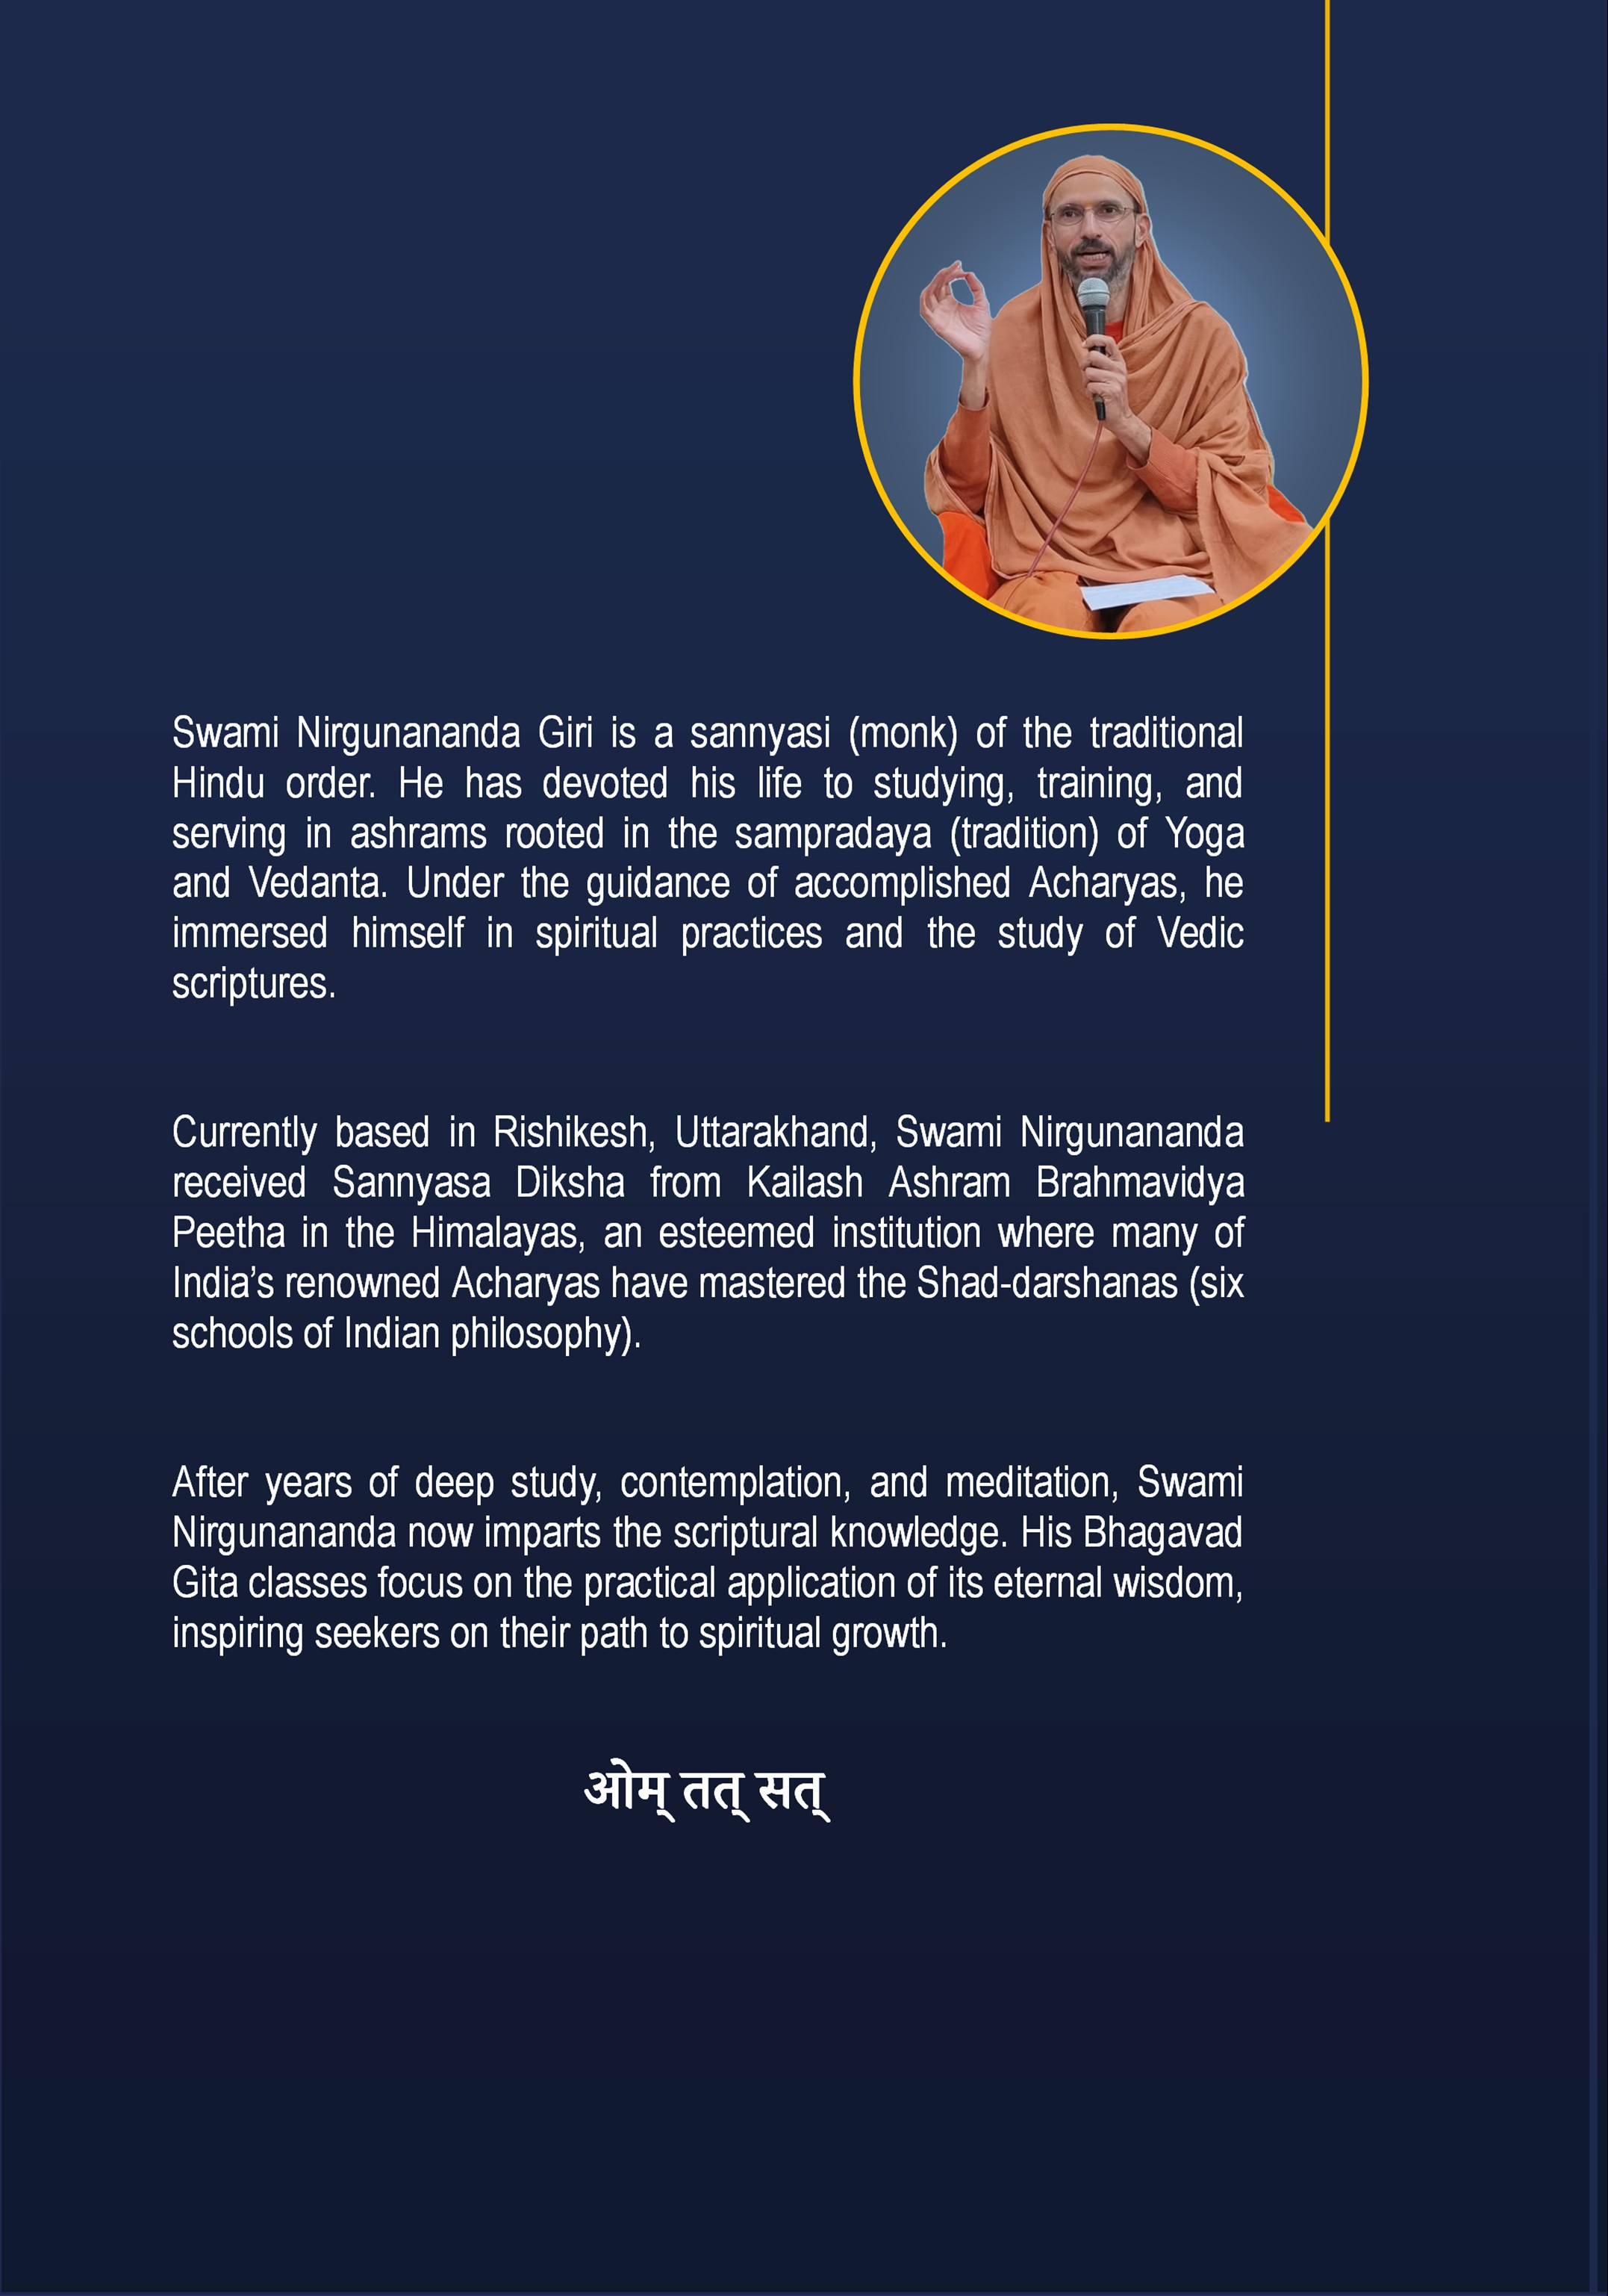
\includegraphics[width=\paperwidth,height=\paperheight]{../images/page02.jpg}%
    }%
	}
   \else% do nothing
   \AddToShipoutPictureBG*{%
    \AtPageLowerLeft{%
        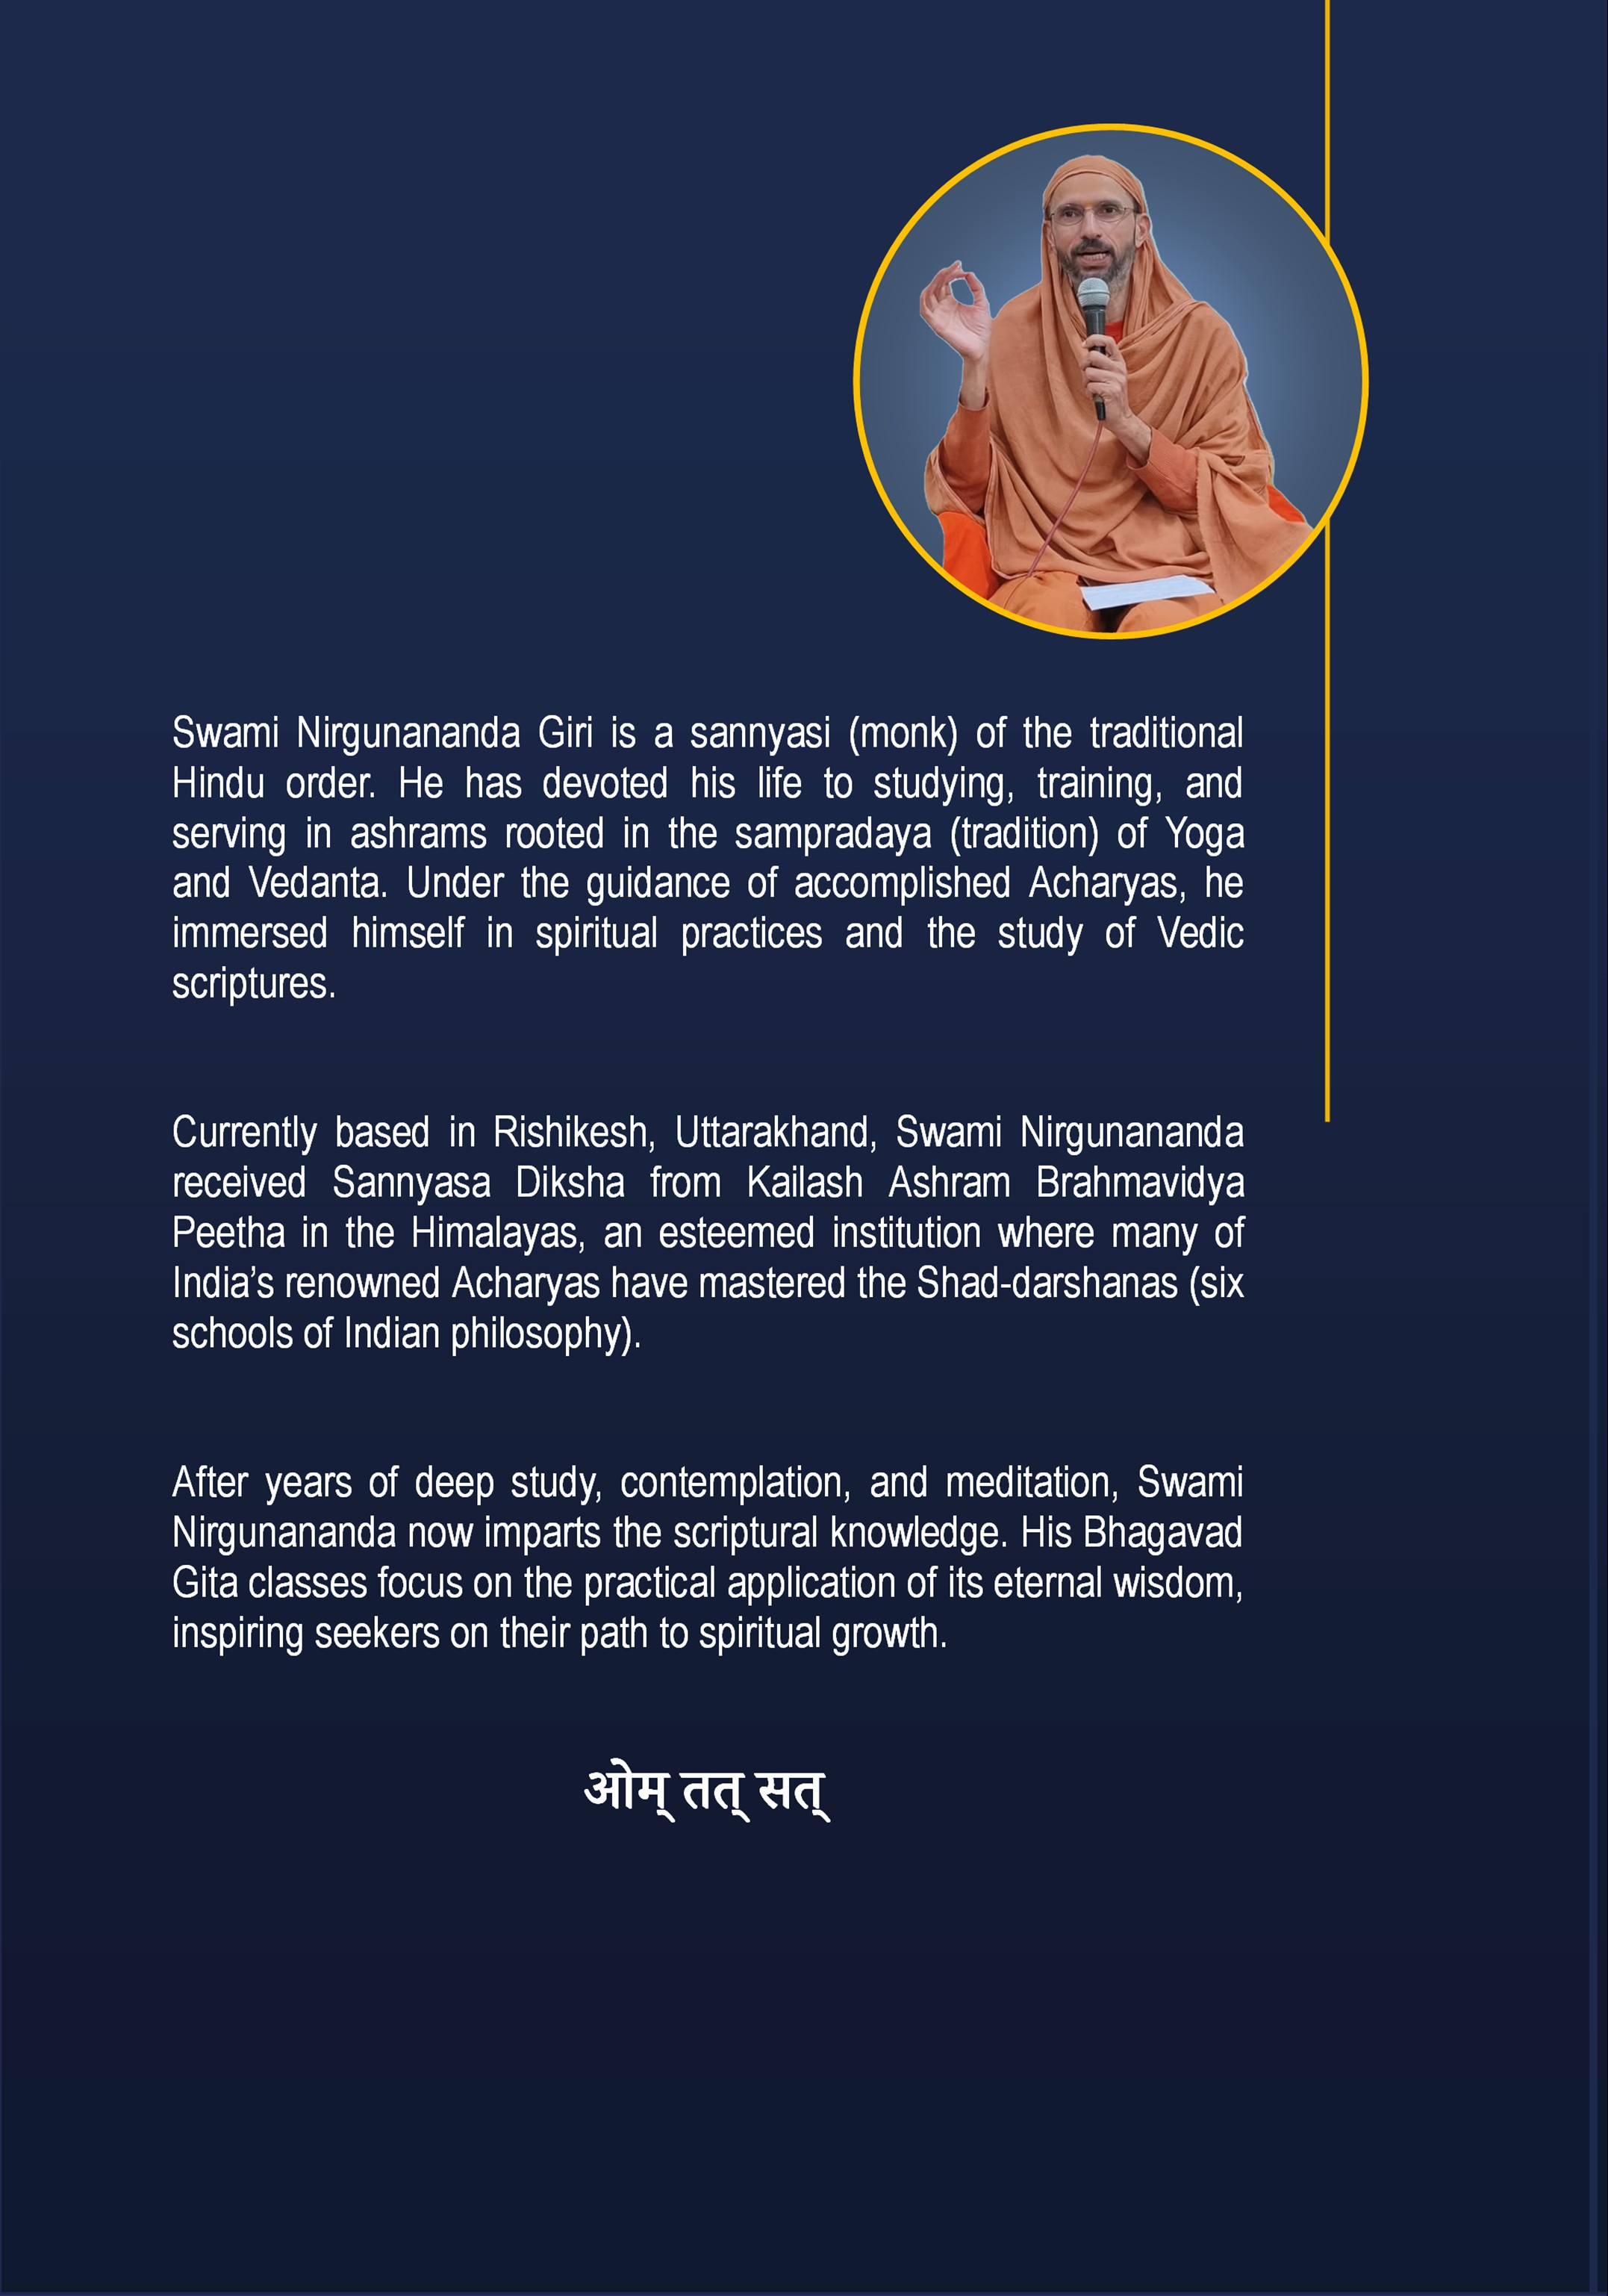
\includegraphics[width=\paperwidth,height=\paperheight]{../images/page02.jpg}%
    }%
	}
\fi
\begin{titlepage}
	%\pagecolor{pastelblue}
	\AddToShipoutPictureBG*{%
    \AtPageLowerLeft{%
        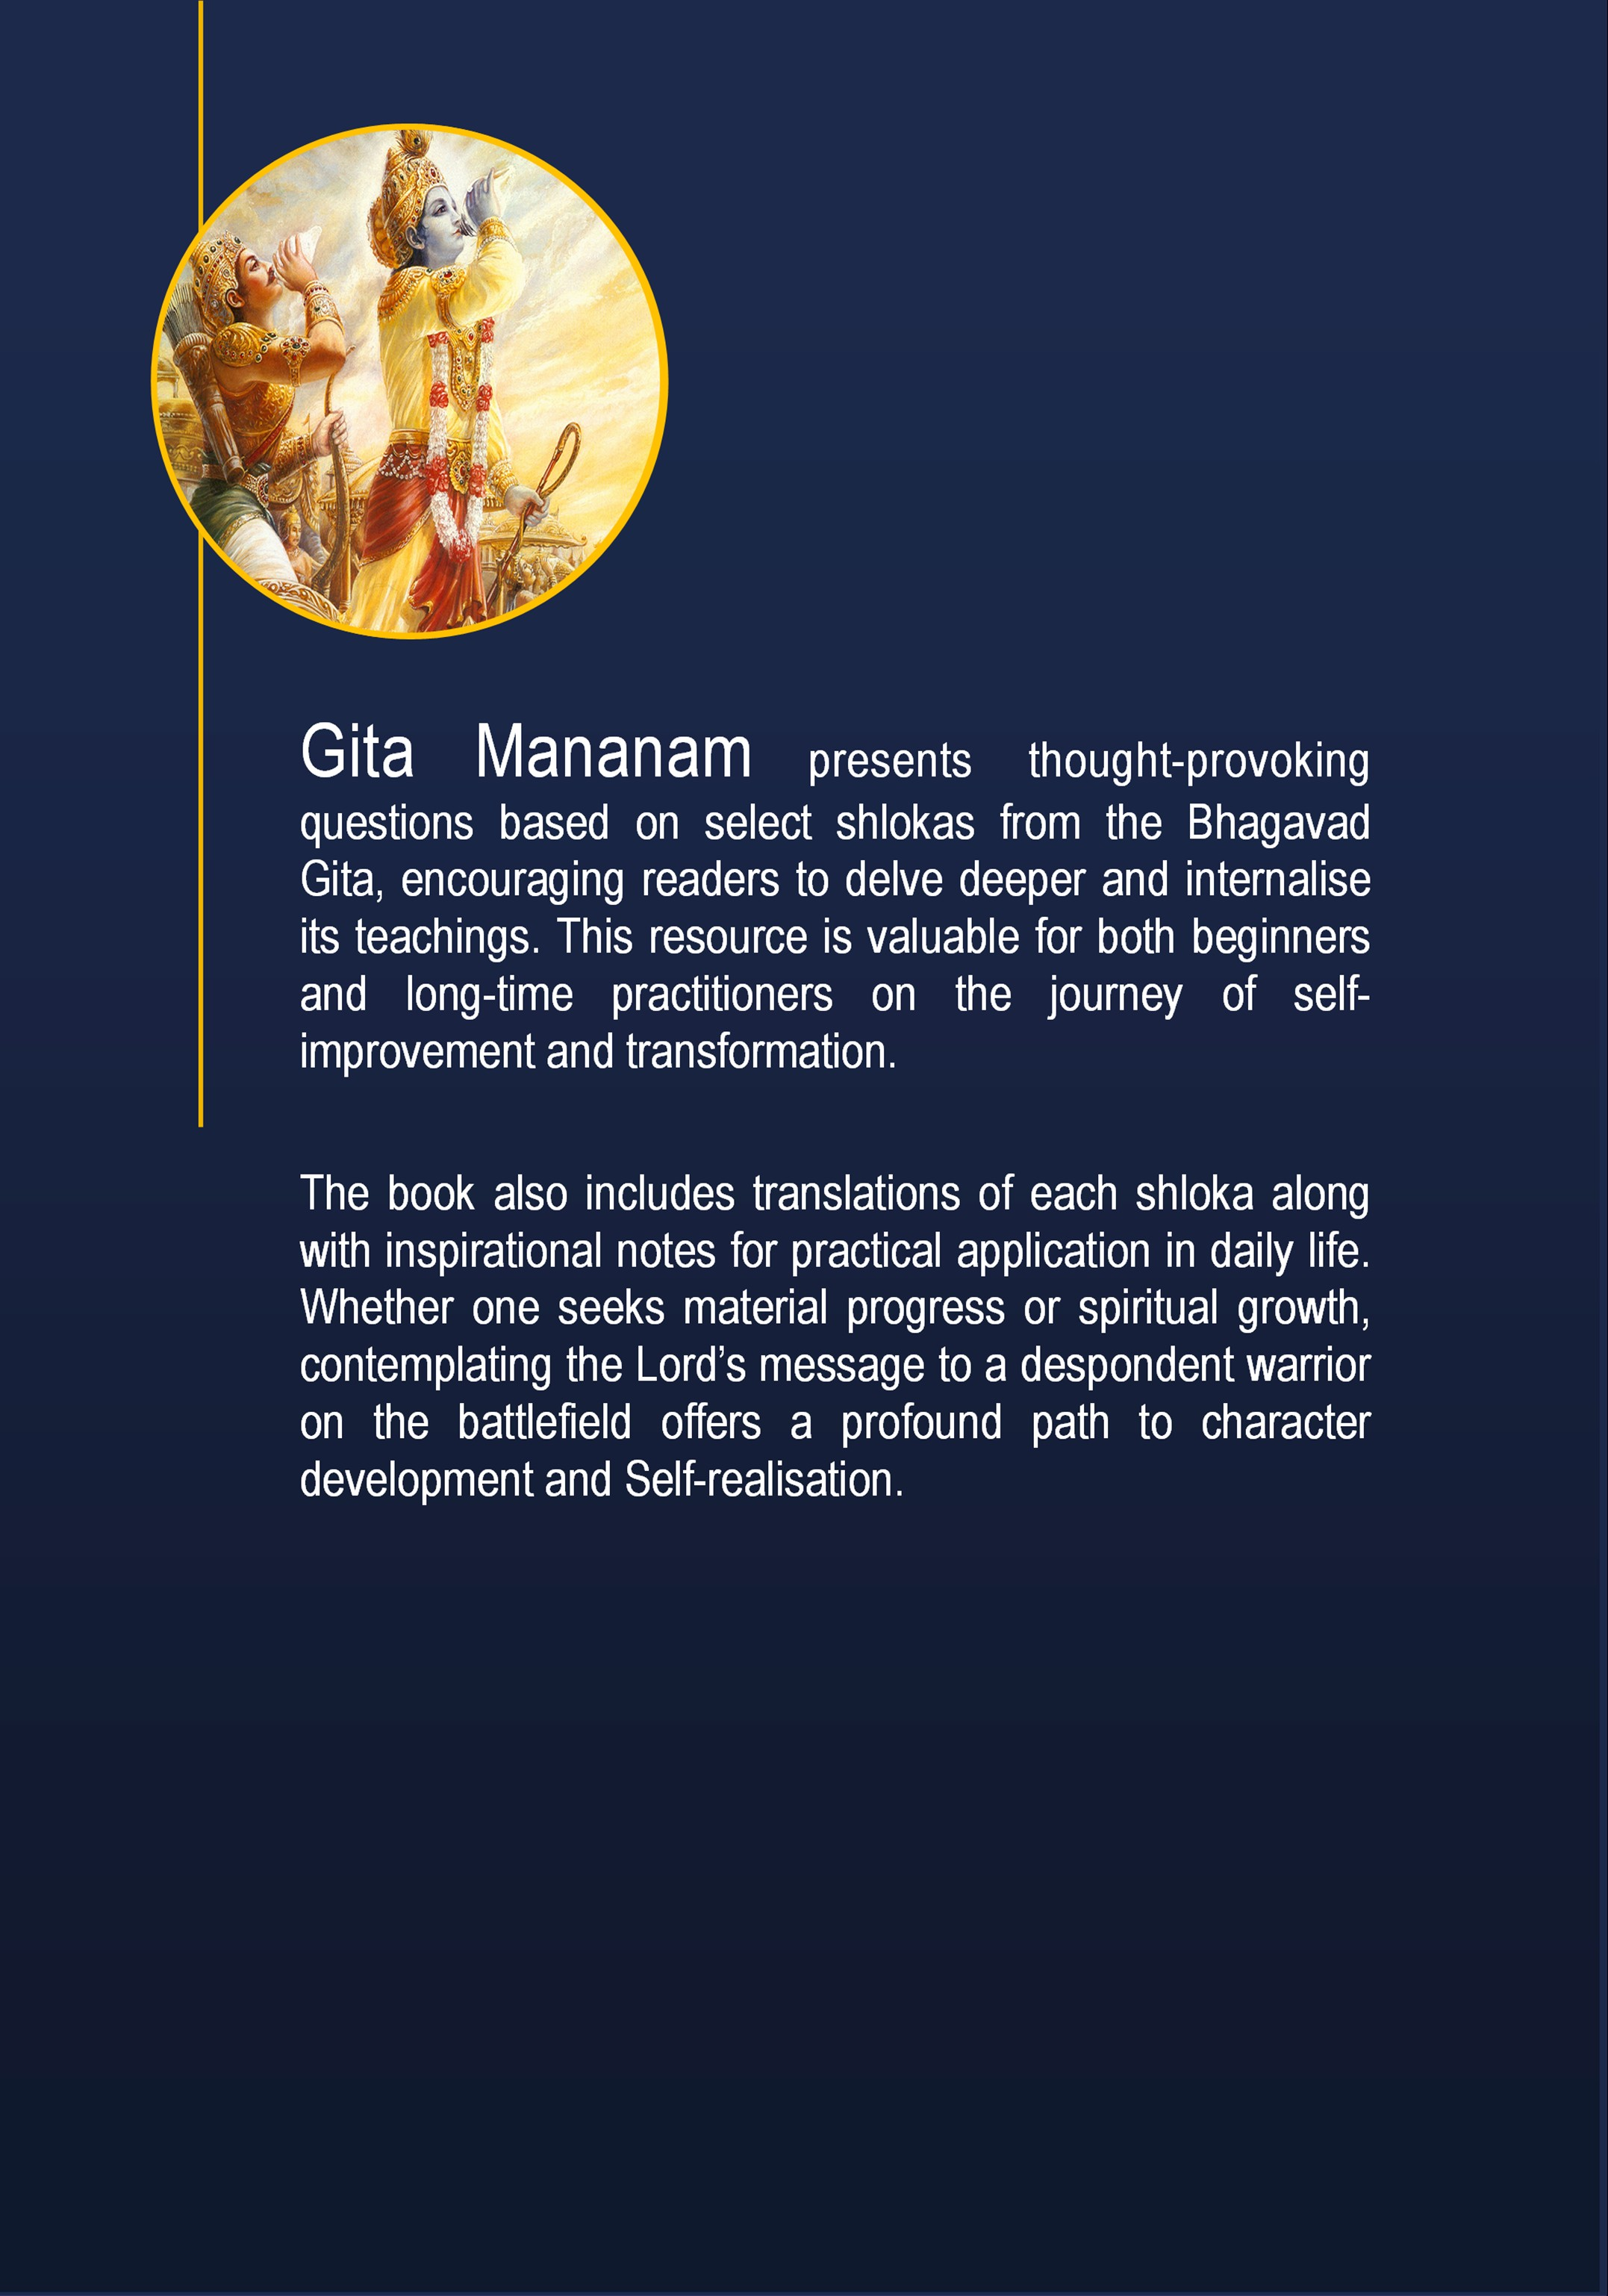
\includegraphics[width=\paperwidth,height=\paperheight]{../images/page03.jpg}%
    }%
}
    \begin{center}
        \vspace*{0.5cm}
            
        {\Huge
        %\textbf{\color{white}\fontsize{50}{60}\selectfont ಗೀತಾ ಮನನಂ}
		}
        %\textbf{\\ \small \color{white}ದೈನಂದಿನ ಸ್ಪೂರ್ತಿ ಹಾಗೂ ಆತ್ಮಾವಲೋಕನಕ್ಕಾಗಿ}    
        \vspace{1.0cm}
            
        
		
            
        \vfill
            
        
            
        \vspace{0.1cm}
        {\color{white}    
		%\textbf{{\Large \mananamfont ಸ್ವಾಮಿ ನಿರ್ಗುಣಾನಂದ ಗಿರಿ}}\\
		%{\normalsize Swami Nirgunananda Giri\\Rishikesh, India}
        }
    \end{center}
\end{titlepage}
\nopagecolor% Use this to restore the color pages to white
\end{document}
